% presentation
\documentclass{beamer}
\usetheme[height=7mm]{Rochester}
\usecolortheme{rose}

% handout

%\documentclass[handout]{beamer}
%\usepackage{pgfpages} \pgfpagesuselayout{8 on 1}[a4paper]

%\documentclass[mathserif]{article}
%\usepackage{beamerarticle}

\usepackage{amsmath}
\usepackage{comment}
\usepackage{amssymb,amsfonts}
\usepackage[T1]{fontenc}
\usepackage{lmodern}
\usepackage{tikz}
%\usepackage{simpsons}
\usepackage{marvosym}
\usepackage{color}
\usepackage{multirow}
\usepackage{pgffor}
\usepackage{pgfplots}
\usepackage[slide,algoruled,titlenumbered,vlined,noend,linesnumbered,]{algorithm2e}

\usefonttheme{structurebold}

\setbeamertemplate{footline}[frame number]
\setbeamertemplate{navigation symbols}{}
\setbeamerfont{smallverb}{size*={73}}
\usefonttheme[onlymath]{serif}
\setbeamertemplate{theorems}[numbered]
\newtheorem{construction}[theorem]{Construction}
\newtheorem{proposition}[theorem]{Proposition}

\AtBeginSection[] {
  \begin{frame}
    \frametitle{Content}
    \tableofcontents[currentsection]
  \end{frame}
  \addtocounter{framenumber}{-1}
}

\usetikzlibrary[shapes.arrows]
\usetikzlibrary{shapes.geometric}
\usetikzlibrary{backgrounds}
\usetikzlibrary{positioning}
\usetikzlibrary{calc}
\usetikzlibrary{intersections}
\usetikzlibrary{fadings}
\usetikzlibrary{decorations.footprints}
\usetikzlibrary{patterns}
\usetikzlibrary{shapes.callouts}
\usetikzlibrary{fit}
%handout

\providecommand{\abs}[1]{\lvert#1\rvert}

\tikzset{every picture/.style={line width=1pt,show background rectangle},background rectangle/.style={fill=blue!10,rounded corners=2ex}}

\newcommand{\Bob}[3]{ \begin{scope}[shift={(#1,#2)},scale=#3]
  \draw (0,0) circle (0.95 and 1);
  \fill (-0.3,-0.1) circle (0.1);
  \fill (+0.3,-0.1) circle (0.1);
  \draw (0.35,-0.5) arc (-70:-110: 1 and 0.4);
  \draw (-0.3,0.5) arc (-10:-80: 0.8 and 0.8);
  \draw (-0.5,0.8) arc (190:255: 2 and 1);
  \draw (-0.7,0.9) -- +(0.2,-0.09) -- +(0.25,0.2);
  \end{scope} }

\newcommand{\Alice}[3]{ \begin{scope}[shift={(#1,#2)},scale=#3]
  \draw (0,0) circle (0.95 and 1);
  \fill (-0.3,-0.1) circle (0.1);
  \fill (+0.3,-0.1) circle (0.1);
  \draw (0.35,-0.5) arc (-70:-110: 1 and 0.4);
  \draw (0.3,1.3) arc (20:-100: 1.4 and 1);
  \draw (0.5,1.3) arc (150:260: 1 and 1);
  \draw (0.41,1.3) circle (0.35);
  \end{scope} }

  \newcommand{\Evil}[3]{ \begin{scope}[shift={(#1,#2)},scale=#3]
    \draw (0,0) circle (0.95 and 1);
    \fill (-0.1,-0.1) -- +(-0.2,-0.1) -- +(-0.4,0.2); %eye
    \fill (0.1,-0.1) -- +(0.2,-0.1) -- +(0.4,0.2);
    \draw (0.35,-0.5) arc (-70:-110: 1 and 0.4);
    %\fill (0.3,-0.5) -- +(-0.1,-0.2) -- +(-0.2,-0.02);
    %\fill (-0.3,-0.5) -- +(0.1,-0.2) -- +(0.2,-0.02);
    \fill (0.3,0.7) -- +(0.5,0.4) -- +(0.4,-0.2); % horn
    \fill (-0.3,0.7) -- +(-0.5,0.4) -- +(-0.4,-0.2);
    %\draw (0.3,1.3) arc (20:-100: 1.4 and 1);
    %\draw (0.5,1.3) arc (150:260: 1 and 1);
    %\draw (0.41,1.3) circle (0.35);
    \end{scope} }

\newcommand{\Charlie}[3]{ \begin{scope}[shift={(#1,#2)},scale=#3]
    \draw (0,0) circle (0.95 and 1);
    \filldraw[fill=black!20] (-0.35,-0.1) circle (0.25);
    \filldraw[fill=black!20] (+0.35,-0.1) circle (0.25);
    %\draw (0.9,0.2) to [bend left] (-0.9,0.2);
    \draw (0.2,0) to [bend left] (-0.2,0);


    %\draw (0.3,0.7) to [bend right] (-0.3,0.7);
    %\draw (0.4,0.5) to [bend right] (-0.4,0.5);
    %\draw (0.35,-0.5) arc (-70:-110: 1 and 0.4);
    \draw (-0.7,-0.6) to [bend right] (0,-0.6) to [bend right] (0.7,-0.6) to [bend right]  (0,-0.5)  to [bend right]  cycle ;
    %\draw (0.3,1.3) arc (20:-100: 1.4 and 1);
    %\draw (0.5,1.3) arc (150:260: 1 and 1);
    %\draw (0.41,1.3) circle (0.35);
    \end{scope} }

\author{Yu Zhang}
\institute{Harbin Institute of Technology}
\date[Crypto'22A]{Cryptography, Autumn, 2022}

%% presentation
\documentclass{beamer}
\usetheme[height=7mm]{Rochester}
\usecolortheme{rose}

% handout

%\documentclass[handout]{beamer}
%\usepackage{pgfpages} \pgfpagesuselayout{8 on 1}[a4paper]

%\documentclass[mathserif]{article}
%\usepackage{beamerarticle}

\usepackage{amsmath}
\usepackage{comment}
\usepackage{amssymb,amsfonts}
\usepackage[T1]{fontenc}
\usepackage{lmodern}
\usepackage{tikz}
%\usepackage{simpsons}
\usepackage{marvosym}
\usepackage{color}
\usepackage{multirow}
\usepackage{pgffor}
\usepackage{pgfplots}
\usepackage[slide,algoruled,titlenumbered,vlined,noend,linesnumbered,]{algorithm2e}

\usefonttheme{structurebold}

\setbeamertemplate{footline}[frame number]
\setbeamertemplate{navigation symbols}{}
\setbeamerfont{smallverb}{size*={73}}
\usefonttheme[onlymath]{serif}
\setbeamertemplate{theorems}[numbered]
\newtheorem{construction}[theorem]{Construction}
\newtheorem{proposition}[theorem]{Proposition}

\AtBeginSection[] {
  \begin{frame}
    \frametitle{Content}
    \tableofcontents[currentsection]
  \end{frame}
  \addtocounter{framenumber}{-1}
}

\usetikzlibrary[shapes.arrows]
\usetikzlibrary{shapes.geometric}
\usetikzlibrary{backgrounds}
\usetikzlibrary{positioning}
\usetikzlibrary{calc}
\usetikzlibrary{intersections}
\usetikzlibrary{fadings}
\usetikzlibrary{decorations.footprints}
\usetikzlibrary{patterns}
\usetikzlibrary{shapes.callouts}
\usetikzlibrary{fit}
%handout

\providecommand{\abs}[1]{\lvert#1\rvert}

\tikzset{every picture/.style={line width=1pt,show background rectangle},background rectangle/.style={fill=blue!10,rounded corners=2ex}}

\newcommand{\Bob}[3]{ \begin{scope}[shift={(#1,#2)},scale=#3]
  \draw (0,0) circle (0.95 and 1);
  \fill (-0.3,-0.1) circle (0.1);
  \fill (+0.3,-0.1) circle (0.1);
  \draw (0.35,-0.5) arc (-70:-110: 1 and 0.4);
  \draw (-0.3,0.5) arc (-10:-80: 0.8 and 0.8);
  \draw (-0.5,0.8) arc (190:255: 2 and 1);
  \draw (-0.7,0.9) -- +(0.2,-0.09) -- +(0.25,0.2);
  \end{scope} }

\newcommand{\Alice}[3]{ \begin{scope}[shift={(#1,#2)},scale=#3]
  \draw (0,0) circle (0.95 and 1);
  \fill (-0.3,-0.1) circle (0.1);
  \fill (+0.3,-0.1) circle (0.1);
  \draw (0.35,-0.5) arc (-70:-110: 1 and 0.4);
  \draw (0.3,1.3) arc (20:-100: 1.4 and 1);
  \draw (0.5,1.3) arc (150:260: 1 and 1);
  \draw (0.41,1.3) circle (0.35);
  \end{scope} }

  \newcommand{\Evil}[3]{ \begin{scope}[shift={(#1,#2)},scale=#3]
    \draw (0,0) circle (0.95 and 1);
    \fill (-0.1,-0.1) -- +(-0.2,-0.1) -- +(-0.4,0.2); %eye
    \fill (0.1,-0.1) -- +(0.2,-0.1) -- +(0.4,0.2);
    \draw (0.35,-0.5) arc (-70:-110: 1 and 0.4);
    %\fill (0.3,-0.5) -- +(-0.1,-0.2) -- +(-0.2,-0.02);
    %\fill (-0.3,-0.5) -- +(0.1,-0.2) -- +(0.2,-0.02);
    \fill (0.3,0.7) -- +(0.5,0.4) -- +(0.4,-0.2); % horn
    \fill (-0.3,0.7) -- +(-0.5,0.4) -- +(-0.4,-0.2);
    %\draw (0.3,1.3) arc (20:-100: 1.4 and 1);
    %\draw (0.5,1.3) arc (150:260: 1 and 1);
    %\draw (0.41,1.3) circle (0.35);
    \end{scope} }

\newcommand{\Charlie}[3]{ \begin{scope}[shift={(#1,#2)},scale=#3]
    \draw (0,0) circle (0.95 and 1);
    \filldraw[fill=black!20] (-0.35,-0.1) circle (0.25);
    \filldraw[fill=black!20] (+0.35,-0.1) circle (0.25);
    %\draw (0.9,0.2) to [bend left] (-0.9,0.2);
    \draw (0.2,0) to [bend left] (-0.2,0);


    %\draw (0.3,0.7) to [bend right] (-0.3,0.7);
    %\draw (0.4,0.5) to [bend right] (-0.4,0.5);
    %\draw (0.35,-0.5) arc (-70:-110: 1 and 0.4);
    \draw (-0.7,-0.6) to [bend right] (0,-0.6) to [bend right] (0.7,-0.6) to [bend right]  (0,-0.5)  to [bend right]  cycle ;
    %\draw (0.3,1.3) arc (20:-100: 1.4 and 1);
    %\draw (0.5,1.3) arc (150:260: 1 and 1);
    %\draw (0.41,1.3) circle (0.35);
    \end{scope} }

\author{Yu Zhang}
\institute{Harbin Institute of Technology}
\date[Crypto'22A]{Cryptography, Autumn, 2022}

%\input{1introduction.tex}
%\input{2perfectlysecret.tex}
%\input{3privatekey.tex}


\title{Introduction}

\begin{document}
\maketitle
\begin{frame}
\frametitle{Outline}
\tableofcontents
\end{frame}
\section{Cryptography and Modern Cryptography}
\begin{frame}\frametitle{What is Cryptography?}
\begin{itemize}
\item \textbf{Cryptography}: from Greek \emph{krypt\'os}, ``hidden, secret''; and \emph{gr\'{a}phin}, ``writing''
\item \textbf{Cryptography}: the art of writing or solving codes.\\ (Concise oxford dictionary 2006)
\item \textbf{Codes}: a system of prearranged signals, especially used to ensure secrecy in transmitting messages. \\ (\emph{code word} in cryptography)
\item \textbf{1980s}: from Classic to Modern; from Military to Everyone
\item \textbf{Modern cryptography}: the scientific study of mathematical techniques for securing digital information, systems, and distributed computations against adversarial attacks
\end{itemize}
\end{frame}
\begin{frame}\frametitle{What is cryptography? [xkcd:504]}
\begin{figure}
\begin{center}
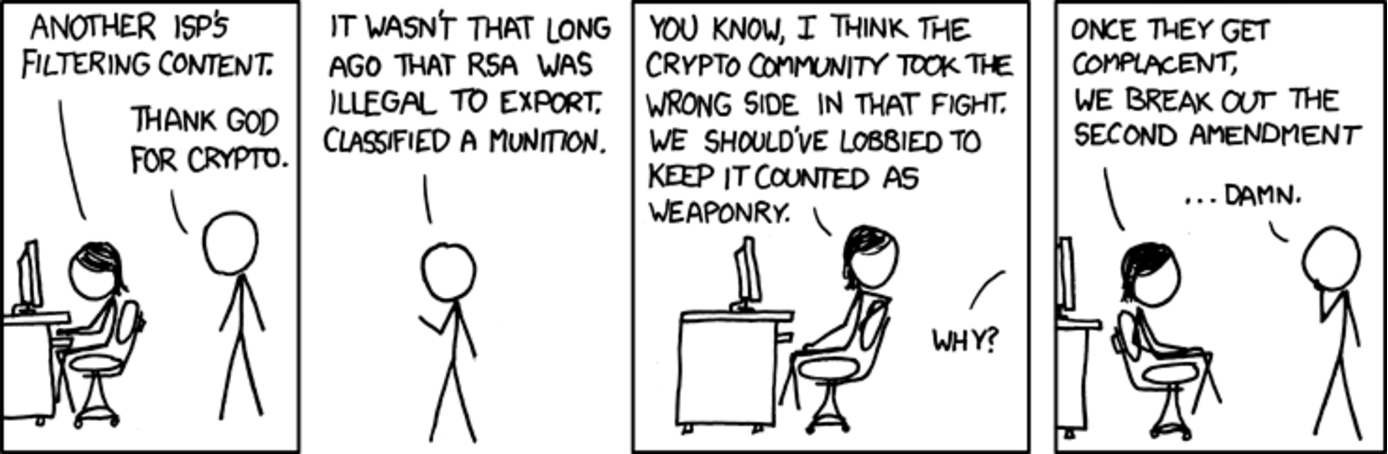
\includegraphics[width=100mm]{pic/legal} 
\end{center}
\end{figure}
\end{frame}
\section{The Setting of Private-Key Encryption}
\begin{frame}\frametitle{Private-Key Encryption}
\begin{itemize}
\item \textbf{Goal}: to construct \textbf{ciphers} (encryption schemes) for providing secret communication between two parties sharing \textbf{private-key} (the symmetric-key) in advance
\item \textbf{Implicit assumption}: there is some way of initially sharing a key in a secret manner
\item \textbf{Disk encryption}: the same user at different points in time
\end{itemize}
\end{frame}
\begin{frame}\frametitle{Alice, Bob  [xkcd:1323]}
Changing the names would be easier, but if you're not comfortable lying, try only making friends with people named Alice, Bob, Carol, etc.
\begin{figure}
\begin{center}
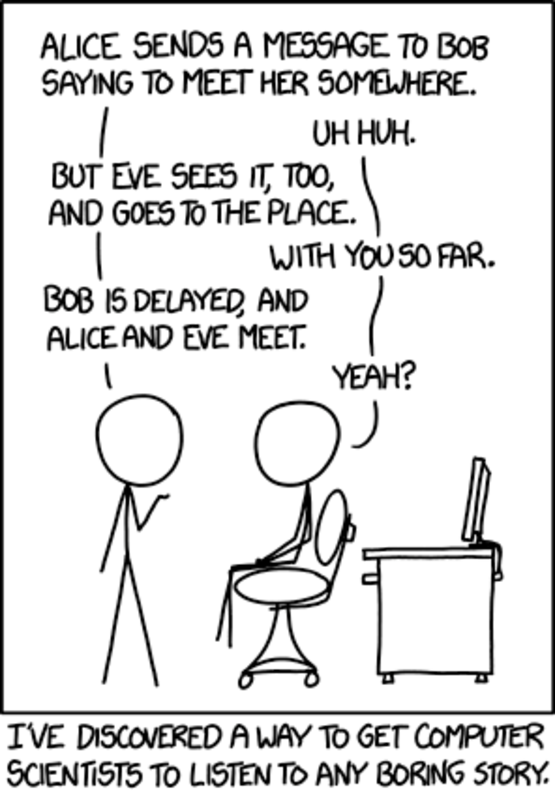
\includegraphics[width=45mm]{pic/alice-bob} 
\end{center}
\end{figure}
\end{frame}
\begin{frame}\frametitle{The Syntax of Encryption}
\begin{figure}
\begin{center}
\begin{tikzpicture}
\node (sender) [minimum size=1cm] {}; \Alice{0}{0}{0.4};
\node (bart) [below of = sender, node distance = 0.7cm] {Alice};
\node (enc) [draw, right of = sender, rounded corners=1ex,node distance = 2cm] {$\mathsf{Enc}$};
\node (k1) [above of = enc, node distance = 1cm] {$k$};
\node (c) [right of = enc, node distance = 2cm] {$c$};
\node (gen) [draw, above of = c, rounded corners=1ex,node distance = 1cm] {$\mathsf{Gen}$};
\node (adv) [below of = c, node distance = 1cm, minimum size=1cm] {}; \Evil{4cm}{-1cm}{0.4};
\node (burns) [below of = adv, node distance = 0.7cm] {Adversary};
\node (dec) [draw, right of = c, rounded corners=1ex,node distance = 2cm] {$\mathsf{Dec}$};
\node (k2) [above of = dec, node distance = 1cm] {$k$};
\node (receiver) [right of = dec, node distance = 2cm, minimum size=1cm] {}; \Bob{8cm}{0}{0.4};
\node (lisa) [below of = receiver, node distance = 0.7cm] {Bob};
\draw[-latex] (sender) -- (enc) node [midway, above] {$m$};
\draw (enc) -- (c); \draw[-latex] (c) -- (dec);
\draw[-latex] (dec) -- (receiver) node [midway, above] {$m$};
\draw[-latex] (k1) -- (enc);
\draw[-latex] (gen) -- (k1);
\draw[-latex] (gen) -- (k2);								
\draw[-latex] (k2) -- (dec);		
\end{tikzpicture}
\end{center}
\end{figure}
\begin{itemize}
\item key $k \in \mathcal{K}$, plaintext (or message) $m \in \mathcal{M}$, ciphertext $c \in \mathcal{C}$
\item \textbf{Key-generation} algorithm~$k \gets \mathsf{Gen}$
\item \textbf{Encryption} algorithm~$c:= \mathsf{Enc}_k(m)$
\item \textbf{Decryption} algorithm~$m:= \mathsf{Dec}_k(c)$
\item \textbf{Encryption scheme}: $\Pi = (\mathsf{Gen}, \mathsf{Enc}, \mathsf{Dec})$
\item \textbf{Basic correctness requirement}: $\mathsf{Dec}_k(\mathsf{Enc}_k(m)) = m$
\end{itemize}
\end{frame}
\begin{frame}\frametitle{Securing Key vs Obscuring Algorithm}
\begin{itemize}
\item Easier to maintain secrecy of a short key
\item In case the key is exposed, easier for the honest parties to change the key
\item In case many pairs of people, easier to use the same algorithm, but different keys
\end{itemize}
\begin{alertblock}{Kerckhoffs's principle}
\begin{quote}
The cipher method must not be required to be secret, and it must be able to fall into the hands of the enemy without inconvenience.
\end{quote}	
\end{alertblock}
\begin{alertblock}{Shannon's maxim}
	\begin{quote}
		The enemy knows the system.
	\end{quote}	
\end{alertblock}
\end{frame}
\begin{frame}\frametitle{Why ``Open Cryptographic Design''}
\begin{itemize}
\item Published designs undergo public scrutiny are to be stronger
\item Better for security flaws to be revealed by ``ethical hackers''
\item Reverse engineering of the code (or leakage by industrial espionage) poses a serious threat to security
\item Enable the establishment of standards.
\end{itemize}
\begin{exampleblock}{Dual EC: A Standardized Back Door}
	``Dual EC was standardized by NIST, ANSI, and ISO among other algorithms to generate pseudorandom numbers.'' ``The Snowden revelations, and in particular reports on Project Bullrun and the SIGINT Enabling Project, have indicated that Dual EC was part of a systematic effort by NSA to subvert standards.'' ``Reuters reported that NSA paid RSA ``\$10 million in a deal that set [Dual EC] as the preferred, or default, method for number generation in the BSafe software.''''	
\end{exampleblock}
\end{frame}
\begin{frame}\frametitle{Attack Scenarios}	
\begin{itemize}
\item \textbf{Ciphertext-only}: the adversary just observes ciphertext
\item \textbf{Known-plaintext}: the adversary learns pairs of plaintexts/ciphertexts under the same key
\item \textbf{Chosen-plaintext}: the adversary has the ability to obtain the encryption of plaintexts of its choice
\item \textbf{Chosen-ciphertext}: the adversary has the ability to obtain the decryption of \textbf{other} ciphertexts of its choice
\item \textbf{Passive attack}: COA KPA
\begin{itemize}
\item because not all ciphertext are confidential
\end{itemize}
\item \textbf{Active attack}: CPA CCA
\begin{itemize}
\item when to encrypt/decrypt whatever an adversary wishes?
\end{itemize}
\end{itemize}	
\end{frame}
\section{Historical Ciphers and Their Cryptanalysis}
\begin{comment}
	\begin{frame}\frametitle{Why We Learn Broken Ciphers?}
	\begin{itemize}
	\item To understand the weaknesses of an ``ad-hoc'' approach
	\item To learn that ``simple'' approaches are unlikely to succeed
	\item To feel that ``we are smart enough to do some crypt-analyzing''
	\end{itemize}
	\end{frame}
\end{comment}

\begin{frame}[fragile]\frametitle{Caesar's Cipher}
\begin{quote}
If he had anything confidential to say, he wrote it in cipher, that is, by so changing the order of the letters of the alphabet, that not a word could be made out. If anyone wishes to \alert{decipher} these, and get at their meaning, he must \alert{substitute the fourth letter of the alphabet, namely D, for A}, and so with the others

\rightline{--Suetonius,``Life of Julius Caesar''}
\end{quote}
\begin{itemize}
	\item $\mathsf{Enc}(m)=m+3\mod 26$ \footnote{In fact the quote indicates that decryption involved rotating letters of the alphabet forward 3 positions, $\mathsf{Dec}(c)=c+3\mod 26$}
	\item \textbf{Weakness}: ? %\alert{What is the key?}
\end{itemize}
\begin{exampleblock}{Example}
\verb|begintheattacknow|
%\verb|EHJLQWKHDWWDFNQRZ|
\end{exampleblock}
\end{frame}
\begin{frame}[fragile]\frametitle{Shift Cipher}
\begin{itemize}
\item $\mathsf{Enc}_k(m)=m+k\mod 26$
\item $\mathsf{Dec}_k(c)=c-k\mod 26$
\item \textbf{Weakness}: ? %Fragile under \textbf{Brute-force attack} (exhaustive search)
\end{itemize}
\begin{exampleblock}{Example: Decipher the string}	
\verb|EHJLQWKHDWWDFNQRZ|
\end{exampleblock}
\begin{alertblock}{Sufficient Key Space Principle}
Any secure encryption scheme must have a key space that is not vulnerable to exhaustive search.\footnote{If the plaintext space is larger than the key space.}
\end{alertblock}
\end{frame}
\begin{frame}\frametitle{Index of Coincidence (IC) Method (to find $k$)}
\textbf{How to automatically determine that the deciphered text makes sense?}

\textbf{Index of Coincidence (IC)}: the probability that two randomly selected letters (pick-then-return) will be identical.

Let $p_i$ denote the probability of $i$th letter in English text.
\[I \overset{\text{def}}{=}\sum_{i=0}^{25} p_i^2 \]
\begin{exampleblock}{Example}
What's the IC of `apple'?
\end{exampleblock}

For a long English text, the IC is $\approx 0.065$.
For $j = 0, 1, \dotsc , 25$, $q_j$ is the probability of $j$th letter in the ciphertext.
\[I_j \overset{\text{def}}{=}\sum_{i=0}^{25} p_i \cdot q_{i+j}\]
\alert{Q: For shift cipher, if $j = k$, then $I_j \approx$ ?}
\end{frame}

\begin{frame}[fragile]\frametitle{Mono-Alphabetic Substitution}
\begin{itemize}
\item \textbf{Idea}: To map each character to a different one in an arbitrary manner
\item \textbf{Strength}: Key space is large $\approx 2^{88}$. \alert{Q: how to count?}
\item \textbf{Weakness}: ? %The mapping of each letter is fixed
\end{itemize}
\begin{exampleblock}{Example}
\verb|abcdefghijklmnopqrstuvwxyz|\\
\verb|XEUADNBKVMROCQFSYHWGLZIJPT|

Plaintext: \verb|tellhimaboutme|\\
Ciphertext: \verb|??????????????|
\end{exampleblock}
\end{frame}
\begin{frame}[fragile]\frametitle{Attack with Statistical Patterns}
\begin{enumerate}
\item Tabulate the frequency of letters in the ciphertext
\item Compare it to those in English text
\item Guess the most frequent letter corresponds to \verb|e|, and so on
\item Choose the plaintext that does ``make sense'' (Not trivial)
\end{enumerate}
\begin{table}
\begin{center}
\caption{Average letter frequencies for English-language text}
\begin{tabular}{|cc|cc|cc|cc|cc|} \hline
e & 12.7\% & t & 9.1\% & a & 8.2\% & o & 7.5\% & i & 7.0\%\\
n & 6.7\% & \_ & 6.4\% & s & 6.3\% & h & 6.1\% & r & 6.0\%\\
d & 4.3\% & l & 4.0\% & c & 2.8\% & u & 2.8\% & m & 2.4\%\\
w & 2.4\% & f & 2.2\% & g & 2.0\% & y & 2.0\% & p & 1.9\%\\
b & 1.5\% & v & 1.0\% & k & 0.8\% & j & 0.2\% & x & 0.2\%\\
q & 0.1\% & z & 0.1\% & & & & & &\\ \hline
\end{tabular}
\end{center}
\end{table}
\end{frame}
\begin{frame}[fragile]\frametitle{Example of Frequency Analysis (Ciphertext)}
\begin{verbatim}
LIVITCSWPIYVEWHEVSRIQMXLEYVEOIEWHRXEXIPFEMVEWHKVS
TYLXZIXLIKIIXPIJVSZEYPERRGERIMWQLMGLMXQERIWGPSRIH
MXQEREKIETXMJTPRGEVEKEITREWHEXXLEXXMZITWAWSQWXSWE
XTVEPMRXRSJGSTVRIEYVIEXCVMUIMWERGMIWXMJMGCSMWXSJO
MIQXLIVIQIVIXQSVSTWHKPEGARCSXRWIEVSWIIBXVIZMXFSJX
LIKEGAEWHEPSWYSWIWIEVXLISXLIVXLIRGEPIRQIVIIBGIIHM
WYPFLEVHEWHYPSRRFQMXLEPPXLIECCIEVEWGISJKTVWMRLIHY
SPHXLIQIMYLXSJXLIMWRIGXQEROIVFVIZEVAEKPIEWHXEAMWY
EPPXLMWYRMWXSGSWRMHIVEXMSWMGSTPHLEVHPFKPEZINTCMXI
VJSVLMRSCMWMSWVIRCIGXMWYMX
\end{verbatim}
\end{frame}
\begin{frame}[fragile]\frametitle{Example of Frequency Analysis (Analysis)}
Count and Guess, Trial and Error.
\begin{table}
\begin{center}
\caption{Analysis Steps}
\begin{tabular}{|r|l|} \hline
Ciphertext & Plaintext \\ \hline
\alert{I}   & \alert{e} \\
\alert{XLI} & \alert{the} \\
\alert{E} & \alert{a} \\
\alert{R}tate & \alert{s}tate \\
atthatt\alert{MZ}e & atthatt\alert{im}e \\
he\alert{V}e & he\alert{r}e \\
remar\alert{A} & remar\alert{k} \\ \hline
\end{tabular}
\end{center}
\end{table}
\end{frame}
\begin{frame}[fragile]\frametitle{Example of Frequency Analysis (Plaintext)}
\begin{quote}
Hereupon Legrand arose, with a grave and stately air, and brought me the beetle
from a glass case in which it was enclosed. It was a beautiful scarabaeus, and, at
that time, unknown to naturalists -- of course a great prize in a scientific point
of view. There were two round black spots near one extremity of the back, and a
long one near the other. The scales were exceedingly hard and glossy, with all the
appearance of burnished gold. The weight of the insect was very remarkable, and,
taking all things into consideration, I could hardly blame Jupiter for his opinion
respecting it.

\rightline{--Edgar Allan Poe's ``The Gold-Bug''}
\end{quote}
\end{frame}

\begin{frame}[fragile]\frametitle{Vigen\`{e}re (poly-alphabetic shift) Cipher}
\begin{itemize}
\item \textbf{Idea}: To ``smooth out'' the distribution in the ciphertext by mapping different instances of the same letter in the plaintext to different ones in the ciphertext
\item \textbf{Encryption}: $c_i=m_i+k_{[i\bmod t]}$, $t$ is the length (period) of $k$
\item \textbf{Cryptanalysis}: Need find $t$; if $t$ is known, need know whether the decryption ``makes sense'', but brute force ($26^t$) is infeasible for $t > 15$
\end{itemize}
\begin{exampleblock}{Example (Key is `cafe')}
\begin{description}[Ciphertext]
\item[Plaintext]  \verb|tellhimaboutme| \\
\item[Key]        \verb|cafecafecafeca| \\
\item[Ciphertext] \verb|??????????????| %\verb|WFRQKJSFEPAYPF|
\end{description}
\end{exampleblock}
\end{frame}
\begin{frame}[fragile]\frametitle{Kasiski's Method (to find $t$)}
\begin{itemize}
\item To identify repeated patterns of length 2 or 3
\item The distance between such appearances is a multiple of $t$
\item $t$ is the greatest common divisor of all the distances
\end{itemize}
\begin{exampleblock}{Example (Key is `beads')}
\begin{semiverbatim}
themanandthewomanretrievedtheletterfromthepostoffice
beadsbeadsbeadsbeadsbeadsbeansdeadsbeadsbeadsbeadbea
VMFQTPFOH\alert{MJJ}XSFCSSIMTNFZXFYISEIYUIKHWPQ\alert{MJJ}QSLVTGJKGF
\end{semiverbatim}
\end{exampleblock}
\end{frame}
\begin{frame}\frametitle{Index of Coincidence (IC) Method (to find $t$)}
For $\tau = 1, 2, \dotsc$, $q_i$ is the probability of $i$th letter in $c_1, c_{1+\tau}, c_{1+2\tau}, \dotsc$, IC is
\[I_\tau \overset{\text{def}}{=}\sum_{i=0}^{25} q_i^2\]
\alert{If $\tau = t$, then $I_\tau \approx ?$} ; otherwise $q_i \approx \frac{1}{26}$ and
\[I_\tau \approx \sum_{i=0}^{25} \left(\frac{1}{26}\right)^2 \approx 0.038\]
Then reuse IC method to find $k_i$.
\begin{alertblock}{Arbitrary Adversary Principle}
Security must be guaranteed for any adversary within the class of adversaries having the specified power
\end{alertblock}
\end{frame}
\begin{frame}\frametitle{Cryptanalytic Attacks (homework assignment)}
\begin{itemize}
\item Under COA, the requirement for ciphertext related to the size of the key space.  Vig\`{e}nere > mono-alphabetic sub. > shift
\item Under KPA, trivially broken.
\end{itemize}
\begin{alertblock}{Lessons learned}
\begin{itemize}
\item Sufficient key space principle
\item Designing secure cipher is a hard task
\item Complexity does not imply security (then what does?)
\item Arbitrary adversary principle
\end{itemize}
\end{alertblock}
\end{frame}
\section{The Basic Principles of Modern Cryptography}
\begin{frame}\frametitle{Three Main Principles of Modern Cryptography}
\begin{enumerate}
\item The formulation of a rigorous \textbf{definition} of security / threat model
\item When the security of a cipher relies on an unproven \textbf{assumption}, this assumption must be precisely stated and be as minimal as possible
\item Cipher should be accompanied by a rigorous \textbf{proof} of security with the above definition and the above assumption
\end{enumerate}
\end{frame}
\begin{frame}\frametitle{Why Principle 1 -- Formulation of Exact Definitions}
\begin{exampleblock}{Q: how would you formalize the security for private-key encryption?}
\begin{enumerate}
\item \emph{No adversary can find the secret key when given a ciphertext.}\\
$\mathsf{Enc}_k(m)=m$
\item \emph{No adversary can find the plaintext that corresponds to the ciphertext.}\\
$\mathsf{Enc}_k(m)=m_{0}\| \mathsf{AES}_k(m)$
\item \emph{No adversary can determine any character of the plaintext that corresponds to the ciphertext.}\\
$m=1000$, someone can learn $ 800 < m < 1200$
\item \emph{No adversary can derive any meaningful information about the plaintext from the ciphertext.}\\
Could you define so-called `meaningful'?
\end{enumerate}
\emph{\alert{Definitions of security should suffice for all potential applications.}}
\end{exampleblock}
\end{frame}
\begin{frame}\frametitle{Why Principle 1 -- How to define}
%\begin{exampleblock}{General Form}
%A cryptographic scheme for a given \textbf{task} is secure if no adversary of a specified \textbf{power} can achieve a specified \textbf{break}
%\end{exampleblock}

How To Define Security -- Lesson From Alan Turing
\begin{itemize}
\item What's computation?\footnote{Q: Any ``mathematical proof that there exist well-defined problems that computers cannot solve''? A: Halting Problem in computability theory}
\begin{enumerate}
\item A direct appeal to \textbf{intuition}
\item A \textbf{proof of the equivalence} of two definitions\\ (The new one has a greater intuitive appeal)
\item Giving \textbf{examples} solved using a definition
\end{enumerate}
\item Additional method for security: \textbf{Test of time}
\end{itemize}
\end{frame}	
\begin{frame}\frametitle{Principle 2 -- Reliance on Precise Assumptions}
Most cryptographic constructions \textbf{cannot be proven secure unconditionally}
\begin{itemize}
	\item \textbf{Why?} 
	\begin{enumerate}
		\item Validation of the assumption
		\item Comparison of schemes
		\item Facilitation of proofs of security
	\end{enumerate}
	\textbf{The construction is secure if the assumption is true.}
	\item \textbf{How?} 
	\begin{enumerate}
		\item old, so well tested
		\item simple and lower-level, so easy to study, refute \& correct
	\end{enumerate}
\end{itemize}
\end{frame}
\begin{frame}\frametitle{Principle 3 -- Rigorous Proofs of Security}
\begin{itemize}
\item \textbf{Why?} Proofs are more desirable in computer security than in other fields.
\item \textbf{The reductionist approach}: 
\begin{theorem}	Given that Assumption X is true, Construction Y is secure according to the given definition.
\end{theorem}
\begin{proof} Reduce the problem given by X to the problem of breaking Y.
\end{proof}
\item \textbf{Ad-hoc approaches}: for those who need a ``quick and dirty'' solution, or who are just simply unaware.
\end{itemize}
\end{frame}
\begin{frame}\frametitle{Summary}
\begin{itemize}
\item Cryptography secures information, transactions and computations
\item Kerckhoffs's principle \& Open cryptographic design
\item Caesar's, shift, Mono-Alphabetic sub., Vigen\`{e}re
\item Brute force, letter frequency, Kasiski's, IC
\item Sufficient key space principle
\item Arbitrary adversary principle
\item Rigorously proven security
\end{itemize}
\end{frame}
\end{document}


%% presentation
\documentclass{beamer}
\usetheme[height=7mm]{Rochester}
\usecolortheme{rose}

% handout

%\documentclass[handout]{beamer}
%\usepackage{pgfpages} \pgfpagesuselayout{8 on 1}[a4paper]

%\documentclass[mathserif]{article}
%\usepackage{beamerarticle}

\usepackage{amsmath}
\usepackage{comment}
\usepackage{amssymb,amsfonts}
\usepackage[T1]{fontenc}
\usepackage{lmodern}
\usepackage{tikz}
%\usepackage{simpsons}
\usepackage{marvosym}
\usepackage{color}
\usepackage{multirow}
\usepackage{pgffor}
\usepackage{pgfplots}
\usepackage[slide,algoruled,titlenumbered,vlined,noend,linesnumbered,]{algorithm2e}

\usefonttheme{structurebold}

\setbeamertemplate{footline}[frame number]
\setbeamertemplate{navigation symbols}{}
\setbeamerfont{smallverb}{size*={73}}
\usefonttheme[onlymath]{serif}
\setbeamertemplate{theorems}[numbered]
\newtheorem{construction}[theorem]{Construction}
\newtheorem{proposition}[theorem]{Proposition}

\AtBeginSection[] {
  \begin{frame}
    \frametitle{Content}
    \tableofcontents[currentsection]
  \end{frame}
  \addtocounter{framenumber}{-1}
}

\usetikzlibrary[shapes.arrows]
\usetikzlibrary{shapes.geometric}
\usetikzlibrary{backgrounds}
\usetikzlibrary{positioning}
\usetikzlibrary{calc}
\usetikzlibrary{intersections}
\usetikzlibrary{fadings}
\usetikzlibrary{decorations.footprints}
\usetikzlibrary{patterns}
\usetikzlibrary{shapes.callouts}
\usetikzlibrary{fit}
%handout

\providecommand{\abs}[1]{\lvert#1\rvert}

\tikzset{every picture/.style={line width=1pt,show background rectangle},background rectangle/.style={fill=blue!10,rounded corners=2ex}}

\newcommand{\Bob}[3]{ \begin{scope}[shift={(#1,#2)},scale=#3]
  \draw (0,0) circle (0.95 and 1);
  \fill (-0.3,-0.1) circle (0.1);
  \fill (+0.3,-0.1) circle (0.1);
  \draw (0.35,-0.5) arc (-70:-110: 1 and 0.4);
  \draw (-0.3,0.5) arc (-10:-80: 0.8 and 0.8);
  \draw (-0.5,0.8) arc (190:255: 2 and 1);
  \draw (-0.7,0.9) -- +(0.2,-0.09) -- +(0.25,0.2);
  \end{scope} }

\newcommand{\Alice}[3]{ \begin{scope}[shift={(#1,#2)},scale=#3]
  \draw (0,0) circle (0.95 and 1);
  \fill (-0.3,-0.1) circle (0.1);
  \fill (+0.3,-0.1) circle (0.1);
  \draw (0.35,-0.5) arc (-70:-110: 1 and 0.4);
  \draw (0.3,1.3) arc (20:-100: 1.4 and 1);
  \draw (0.5,1.3) arc (150:260: 1 and 1);
  \draw (0.41,1.3) circle (0.35);
  \end{scope} }

  \newcommand{\Evil}[3]{ \begin{scope}[shift={(#1,#2)},scale=#3]
    \draw (0,0) circle (0.95 and 1);
    \fill (-0.1,-0.1) -- +(-0.2,-0.1) -- +(-0.4,0.2); %eye
    \fill (0.1,-0.1) -- +(0.2,-0.1) -- +(0.4,0.2);
    \draw (0.35,-0.5) arc (-70:-110: 1 and 0.4);
    %\fill (0.3,-0.5) -- +(-0.1,-0.2) -- +(-0.2,-0.02);
    %\fill (-0.3,-0.5) -- +(0.1,-0.2) -- +(0.2,-0.02);
    \fill (0.3,0.7) -- +(0.5,0.4) -- +(0.4,-0.2); % horn
    \fill (-0.3,0.7) -- +(-0.5,0.4) -- +(-0.4,-0.2);
    %\draw (0.3,1.3) arc (20:-100: 1.4 and 1);
    %\draw (0.5,1.3) arc (150:260: 1 and 1);
    %\draw (0.41,1.3) circle (0.35);
    \end{scope} }

\newcommand{\Charlie}[3]{ \begin{scope}[shift={(#1,#2)},scale=#3]
    \draw (0,0) circle (0.95 and 1);
    \filldraw[fill=black!20] (-0.35,-0.1) circle (0.25);
    \filldraw[fill=black!20] (+0.35,-0.1) circle (0.25);
    %\draw (0.9,0.2) to [bend left] (-0.9,0.2);
    \draw (0.2,0) to [bend left] (-0.2,0);


    %\draw (0.3,0.7) to [bend right] (-0.3,0.7);
    %\draw (0.4,0.5) to [bend right] (-0.4,0.5);
    %\draw (0.35,-0.5) arc (-70:-110: 1 and 0.4);
    \draw (-0.7,-0.6) to [bend right] (0,-0.6) to [bend right] (0.7,-0.6) to [bend right]  (0,-0.5)  to [bend right]  cycle ;
    %\draw (0.3,1.3) arc (20:-100: 1.4 and 1);
    %\draw (0.5,1.3) arc (150:260: 1 and 1);
    %\draw (0.41,1.3) circle (0.35);
    \end{scope} }

\author{Yu Zhang}
\institute{Harbin Institute of Technology}
\date[Crypto'22A]{Cryptography, Autumn, 2022}

%\input{1introduction.tex}
%\input{2perfectlysecret.tex}
%\input{3privatekey.tex}


\title{Perfectly Secret Encryption}

\begin{document}
\maketitle
\begin{frame}\frametitle{Outline}
\tableofcontents
\end{frame}
\section{Definitions and Basic Properties}
\begin{frame}\frametitle{Recall The Syntax of Encryption}
\begin{figure}
\begin{center}
\begin{tikzpicture}
\node (sender) [minimum size=1cm] {}; \Alice{0}{0}{0.4};
\node (bart) [below of = sender, node distance = 0.7cm] {Alice};
\node (enc) [draw, right of = sender, rounded corners=1ex,node distance = 2cm] {$\mathsf{Enc}$};
\node (k1) [above of = enc, node distance = 1cm] {$k$};
\node (c) [right of = enc, node distance = 2cm] {$c$};
\node (gen) [draw, above of = c, rounded corners=1ex,node distance = 1cm] {$\mathsf{Gen}$};
\node (adv) [below of = c, node distance = 1cm, minimum size=1cm] {}; \Evil{4cm}{-1cm}{0.4};
\node (burns) [below of = adv, node distance = 0.7cm] {Adversary};
\node (dec) [draw, right of = c, rounded corners=1ex,node distance = 2cm] {$\mathsf{Dec}$};
\node (k2) [above of = dec, node distance = 1cm] {$k$};
\node (receiver) [right of = dec, node distance = 2cm, minimum size=1cm] {}; \Bob{8cm}{0}{0.4};
\node (lisa) [below of = receiver, node distance = 0.7cm] {Bob};
\draw[-latex] (sender) -- (enc) node [midway, above] {$m$};
\draw (enc) -- (c); \draw[-latex] (c) -- (dec);
\draw[-latex] (dec) -- (receiver) node [midway, above] {$m$};
\draw[-latex] (k1) -- (enc);
\draw[-latex] (gen) -- (k1);
\draw[-latex] (gen) -- (k2);								
\draw[-latex] (k2) -- (dec);		
\end{tikzpicture}
\end{center}
\end{figure}
\begin{itemize}
\item $k \in \mathcal{K}, m \in \mathcal{M}, c \in \mathcal{C}$.
\item $k \gets \mathsf{Gen}, c:= \mathsf{Enc}_k(m), m:= \mathsf{Dec}_k(c)$.
\item \textbf{Encryption scheme}: $\Pi = (\mathsf{Gen}, \mathsf{Enc}, \mathsf{Dec})$.
\item \textbf{Random Variable}: $K, M, C$ for key, plaintext, ciphertext.
\item \textbf{Probability}: $\Pr[K=k], \Pr[M=m], \Pr[C=c].$
\item \alert{What's the basic correctness requirement?}
\end{itemize}
\end{frame}
\begin{frame}\frametitle{Definition of `Perfect Secrecy'}
\textbf{Intuition}: An adversary knows the probability distribution over $\mathcal{M}$. $c$ should have no effect on the knowledge of the adversary; the a \emph{posteriori} likelihood that some $m$ was sent should be no different from the a \emph{priori} probability that $m$ would be sent. 
\begin{definition}
$\Pi$ over $\mathcal{M}$ is \textbf{perfectly secret} if for every probability distribution over $\mathcal{M}$, $\forall m \in \mathcal{M}$ and $\forall c \in \mathcal{C}$ for which $\Pr[C = c] > 0$:
\[ \Pr[M=m | C=c] = \Pr[M=m].\]
\end{definition}
\textbf{Simplify}: non-zero probabilities for $\forall m \in \mathcal{M}$ and $\forall c \in \mathcal{C}$.\\

\begin{exampleblock}{Is the below scheme perfectly secret?}{ For $\mathcal{M}=\mathcal{K} = \{ 0,1 \} , \mathsf{Enc}_k(m)= m \oplus k$.}\end{exampleblock}
\end{frame}

\begin{frame}\frametitle{Perfect Secrecy On One Bit}

\begin{exampleblock}{XORing one bit is perfectly secret.}
Let $\Pr[M=1] = p$ and $\Pr[M=0] = 1-p$.
Let us consider a case that $M=1$ and $C=1$.
\[ \Pr[M=1 | C=1] = \Pr[C=1 | M=1 ] \cdot \Pr[ M=1 ] / \Pr[C=1] \]
\[ = \frac{\Pr[K = 1\oplus 1] \cdot p }{ \Pr[C=1 | M=1] \cdot \Pr[M=1] + \Pr[C=1 | M=0] \cdot \Pr[M=0]} \]
\[ = \frac{1/2 \cdot p }{ 1/2 \cdot p + 1/2 \cdot (1-p)} = p = \Pr[M=1] \]
We can do the same for other cases.
\end{exampleblock}
Note that $\Pr[M=1 | C=1] \neq \Pr[M=1, C=1] = \Pr[C=1 | M=1] \cdot \Pr[M=1] = 1/2 \cdot p$.
\end{frame}

\begin{frame}\frametitle{An Equivalent Formulation}
\begin{lemma} \label{lem:ps} 
$\Pi$ over $\mathcal{M}$ is perfectly secret $\iff$ for every probability distribution over $\mathcal{M}$, $\forall m \in \mathcal{M}$ and $\forall c \in \mathcal{C}$:
\[ \Pr[C=c | M=m] = \Pr[C=c].\]
\end{lemma}
\begin{proof}
$\Leftarrow$: Multiplying both sides by $\Pr[M=m]/\Pr[C=c]$, then use Bayes' Theorem.\footnote{If $\Pr[B]\neq 0$ then $ \Pr[A|B] = \left( \Pr[A] \cdot \Pr[B|A] \right) / \Pr[B] $} \\
$ \Pr[C=c | M=m] \cdot \Pr[M=m] / \Pr[C=c] = \Pr[M=m]$\\
$ \Pr[M=m | C=c] \cdot \Pr[C=c] / \Pr[C=c] = \Pr[M=m | C=c]$
$\Rightarrow$: Multiplying both sides by $\Pr[C=c]/\Pr[M=m]$, then use Bayes' Theorem.
\end{proof}
\end{frame}
\begin{frame}\frametitle{Perfect Indistinguishability}
\begin{lemma}\label{lem:pi}
$\Pi$ over $\mathcal{M}$ is perfectly secret $\iff$ for every probability distribution over $\mathcal{M}$, $\forall m_0, m_1 \in \mathcal{M}$ and $\forall c \in \mathcal{C}$:
\[ \Pr[C=c | M=m_0] = \Pr[C=c | M=m_1].\]
\end{lemma}
\begin{proof}
$\Rightarrow$: By Lemma \ref{lem:ps}: $\Pr[C=c | M=m] = \Pr[C=c]$. \\
$\Leftarrow$: $p \overset{\text{def}}{=} \Pr[C=c | M=m_0]$.
\[
\begin{split}
	\Pr[C=c] &= \sum_{m \in \mathcal{M}} \Pr[C=c|M=m] \cdot \Pr[M=m] \\
	&= \sum_{m \in \mathcal{M}} p \cdot \Pr[M=m] = p = \Pr[C=c|M=m_0].
\end{split}
\]
\end{proof}
\end{frame}
\section{The One-Time Pad (Vernam's Cipher)}
\begin{frame}\frametitle{One-Time Pad (Vernam's Cipher)}
\begin{itemize}
	\item $\mathcal{M} = \mathcal{K} = \mathcal{C} = \{0,1\}^{\ell}$.
	\item $\mathsf{Gen}$ chooses a $k$ randomly with probability exactly $2^{-\ell}$.
	\item $c := \mathsf{Enc}_k(m) = k \oplus m$. 
	\item $m := \mathsf{Dec}_k(c) = k \oplus c$. 
\end{itemize}
\begin{theorem}
The one-time pad encryption scheme is perfectly-secret.
\end{theorem}
\begin{proof}
\[\begin{split} \Pr[C=c|M=m] &= \Pr[M \oplus K=c|M=m] \\
&= \Pr[m \oplus K=c] = \Pr[K = m \oplus c] = 2^{-\ell}.
\end{split}
\]
Then Lemma \ref{lem:pi}: $\Pr[C=c | M=m_0] = \Pr[C=c | M=m_1]$.
\end{proof}
\end{frame}
\section{Limitations of Perfect Secrecy}
\begin{frame}\frametitle{Limitations of OTP and Perfect Secrecy}
Key $k$ is as long as $m$, difficult to store and share $k$.
\begin{theorem}
Let $\Pi$ be perfectly-secret over $\mathcal{M}$, and let $\mathcal{K}$ be determined by $\mathsf{Gen}$. Then $|\mathcal{K}|\ge |\mathcal{M}|$. 
\end{theorem}
\begin{proof}
Assume $|\mathcal{K}| < |\mathcal{M}|$.
$\mathcal{M}(c) \overset{\text{def}}{=} \{ \hat{m} | \hat{m} = \mathsf{Dec}_k(c)\  \text{for some}\ \hat{k} \in \mathcal{K} \}$. Since for one $k$, there is at most one $m$ such that $m = \mathsf{Dec}_k(c)$, $|\mathcal{M}(c)|\le |\mathcal{K}| < |\mathcal{M}|$. So $\exists m' \notin \mathcal{M}(c)$. Then
\[ \Pr[M=m'|C=c] = 0 \neq \Pr[M = m'] \]
and so not perfectly secret.
\end{proof}
\end{frame}
\begin{frame}\frametitle{Two Time Pad: Real World Cases}
Only used once for the same key, otherwise
\[c\oplus c'=(m\oplus k)\oplus (m'\oplus k)=m\oplus m'.\]
Learn $m$ from $m\oplus m'$ due to the redundancy of language.
\begin{exampleblock}{MS-PPTP (Win NT)}
\begin{figure}
\begin{center}
\begin{tikzpicture}
\node (sender) [minimum size=1cm,label=below:Client, label=above:$k$] {}; \Alice{0}{0}{0.4};
\node (c) at ($(sender)+(4cm,0.5cm)$) {$\left[ m_1\|m_2\|m_3\right] \oplus PRG(k)$};
\node (c1) [below of = c, node distance = 1cm] {$\left[s_1\|s_2\|s_3\right] \oplus PRG(k)$};
\node (receiver) at ($(sender)+(8cm,0)$) [minimum size=1cm,label=below:Server, label=above:$k$] {}; \Bob{8cm}{0}{0.4};
\draw[-latex] (sender.east |- c) -- (c) -- (receiver.west |- c);
\draw[-latex] (receiver.west |- c1) -- (c1) -- (sender.east |- c1);
\end{tikzpicture}
\end{center}
\end{figure}
Improvement: use two keys for C-to-S and S-to-C separately.
\end{exampleblock}
\end{frame}
\section{Shannon's Theorem}
\begin{frame}\frametitle{Shannon's Theorem}
\begin{theorem}
For $|\mathcal{M}| = |\mathcal{K}| = |\mathcal{C}|$, $\Pi$ is perfectly secret $\iff$
\begin{enumerate}
\item Every $k \in \mathcal{K}$ is chosen with probability $1/|\mathcal{K}|$ by $\mathsf{Gen}$.
\item $\forall m \in \mathcal{M}$ and $\forall c \in \mathcal{C}$, $\exists$ unique $k \in \mathcal{K}$: $c := \mathsf{Enc}_k(m)$.
\end{enumerate}
\end{theorem}
\begin{proof}
$\Leftarrow$: $\Pr[C=c|M=m]=1/|\mathcal{K}|$, use Lemma \ref{lem:pi}. \\
$\Rightarrow (2)$: At least one $k$, otherwise $\Pr[C=c|M=m]=0$; \\
at most one $k$, because $\{\mathsf{Enc}_k(m)\}_{k\in \mathcal{K}} = \mathcal{C}$ and $|\mathcal{K}| = |\mathcal{C}|$.\\
$\Rightarrow (1)$: $k_i$ is such that $\mathsf{Enc}_{k_i}(m_i)=c$.
\[ \begin{split}
\Pr[M = m_i] &= \Pr[M=m_i|C=c] \\
             &= \left( \Pr[C =c|M=m_i] \cdot \Pr[M = m_i] \right) / \Pr[C=c] \\
 &= \left( \Pr[K=k_i] \cdot \Pr[M = m_i] \right) / \Pr[C=c],
\end{split}
\]
so $\Pr[K=k_i] = \Pr[C = c] = 1/|\mathcal{K}|$.
\end{proof}
\end{frame}

\begin{frame}\frametitle{Application of Shannon's Theorem}
\begin{exampleblock}{Is the below scheme perfectly secret?}
Let $\mathcal{M} = \mathcal{C} = \mathcal{K} = \{ 0, 1, 2,\dots , 255 \} $\\
$\mathsf{Enc}_k(m) = m  + k \mod 256$\\
$\mathsf{Dec}_k(c) = c - k \mod 256$
\end{exampleblock}
\end{frame}
\section{Eavesdropping Indistinguishability}
\begin{frame}\frametitle{Eavesdropping Indistinguishability Experiment}
$\mathsf{PrivK}^{\mathsf{eav}}_{\mathcal{A},\Pi}$ denote a \textbf{priv}ate-\textbf{k}ey encryption experiment for a given $\Pi$ over $\mathcal{M}$ and an \textbf{eav}esdropping adversary $\mathcal{A}$.
\begin{enumerate}
	\item $\mathcal{A}$ outputs a pair of messages $m_0, m_1 \in \mathcal{M}$.
	\item $k \gets \mathsf{Gen}$, a random bit $b \gets \{0,1\}$ is chosen. Then $c \gets \mathsf{Enc}_k(m_b)$ is given to $\mathcal{A}$.
	\item $\mathcal{A}$ outputs a bit $b'$
	\item If $b' = b$, $\mathcal{A}$ succeeded $\mathsf{PrivK}^{\mathsf{eav}}_{\mathcal{A},\Pi}=1$, otherwise 0.
\end{enumerate}
\begin{figure}
\begin{center}
\begin{tikzpicture}
%\node (A) at (0,0) {\Homer};
%\node (B) [right of = A, node distance = 4cm] {\Left\Burns};
\node (A) at (0,0) [minimum size=1cm] {}; \Charlie{0}{0}{0.4};
\node (B) [right of = A, node distance = 4cm, minimum size=1cm] {}; \Evil{4cm}{0}{0.4};
\node (1a) [below of=A, node distance=1cm] {};
\node (1b) [below of=B, node distance=1cm] {$m_0, m_1$};
\draw[-latex] (1b) -- (1a) node [midway,above] {};
\node (2a) [below of=1a, node distance=0.5cm] {Gen $b, k$};
\node (2b) [below of=1b, node distance=0.5cm] {};
%\draw[-latex] (2b) -- (2a) node [midway,above] {};
%\node (3a) [below of=2a, node distance=0.5cm] {};
%\node (3b) [below of=2b, node distance=0.5cm] {};
\node (4a) [below of=2a, node distance=0.5cm] {$\mathsf{Enc}_k(m_b)$};
\node (4b) [below of=2b, node distance=0.5cm] {};
\draw[-latex] (4a) -- (4b) node [midway,above] {};
\node (5a) [below of=4a, node distance=0.5cm] {};
\node (5b) [below of=4b, node distance=0.5cm] {$b'$};
\draw[-latex] (5b) -- (5a) node [midway,above] {};
\node (6a) [below of=5a, node distance=0.5cm] {};
\node (6b) [below of=5b, node distance=0.5cm] {};
\node (result) [right of = 6a, node distance = 2cm] {Win if $b = b'$};
\end{tikzpicture}

\end{center}
\end{figure}
\end{frame}
\begin{frame}\frametitle{Adversarial Indistinguishability}
\begin{definition}
$\Pi$ over $\mathcal{M}$ is \textbf{perfectly secret} if for every $\mathcal{A}$ it holds that
\[ \Pr[\mathsf{PrivK}^{\mathsf{eav}}_{\mathcal{A},\Pi}=1] = \frac{1}{2}.\]
\end{definition}
\begin{exampleblock}{Which in the below schemes are perfectly secret?}
\begin{itemize}
\item $\mathsf{Enc}_{k,k'}(m)= \mathsf{OTP}_k(m) \| \mathsf{OTP}_{k'}(m)$
\item $\mathsf{Enc}_{k}(m)= reverse(\mathsf{OTP}_k(m))$
\item $\mathsf{Enc}_{k}(m)= \mathsf{OTP}_k(m) \| k$
%To break semantic security, an attacker would read the secret key from the challenge ciphertext and use it to decrypt the challenge ciphertext. Basically, any ciphertext reveals the secret key.
\item $\mathsf{Enc}_{k}(m)= \mathsf{OTP}_k(m) \| \mathsf{OTP}_k(m) $
\item $\mathsf{Enc}_{k}(m)= \mathsf{OTP}_{0^{n}}(m)$
%To break semantic security, an attacker would ask for the encryption of $0^n$ and $1^n$ and can easily distinguish EXP(0) from EXP(1) because it knows the secret key, namely 0n.
\item $\mathsf{Enc}_{k}(m)= \mathsf{OTP}_k(m) \| LSB(m)$
%To break semantic security, an attacker would ask for the encryption of $0^n$ and $0^{n-1}1$ and can distinguish EXP(0) from EXP(1).
\end{itemize}
\end{exampleblock}
\end{frame}

\begin{frame}\frametitle{Summary}
\begin{itemize}
\item Perfect secrecy $=$ Perfect indistinguishability $=$ Adversarial indistinguishability
\item Perfect secrecy is attainable. The One-Time Pad (Vernam's cipher)
\item Shannon's theorem
\end{itemize}	
\end{frame}
\end{document}

%\input{3privatekey.tex}


\title{Public-Key Encryption Theory}

\begin{document}
\maketitle
\begin{frame}
\frametitle{Outline}
\tableofcontents
\end{frame}
\section{Definitions and Securities of Public-Key Encryption}
\begin{frame}\frametitle{Limitations of Private-Key Cryptography}
\begin{itemize}
\item The key-distribution need physically meeting.
\item The number of keys for $U$ users is $\Theta(U^2)$.
\item Secure communication in open system:
\end{itemize}
\vspace{0.5cm}
Solutions that are based on private-key cryptography are not sufficient to deal with the problem of secure communication in open systems where parties cannot physically meet, or where parties have transient interactions.
\end{frame}
\begin{frame}\frametitle{Needham-Schroeder Protocol for  Symmetric Key}
\begin{itemize}
\item Key Distribution Center (KDC) as Trusted Third Party (TTP), which has the shared key with Alice, and with Bob, respectively.
\item $E_{Bob}(k)$ is a \textbf{ticket} to access $Bob$, $k$ is \textbf{session key}.
\item Used in MIT's Kerberos protocol (in Windows).
\end{itemize}
\begin{columns}[t]
\begin{column}{5cm}
\begin{figure}[t]
\begin{center}
\begin{tikzpicture}[font=\footnotesize,scale=0.7, every node/.style={scale=0.7}]
%\node (A) at (0,0) [label=below:Alice] {\Lisa};
%\node (B) [right of = A, node distance = 4cm,label=below:Bob] {\Left\Bart};
\node (A) at (0,0) [minimum size=1.5cm] {}; \Alice{0}{0}{0.4}; \node at (0,-0.7) {Alice};
\node (B) [right of = A, node distance = 4cm, minimum size=1cm] {}; \Bob{4cm}{0}{0.4}; \node at (4cm,-0.7) {Bob};
\node (KDC) at (2,4) [rounded corners=1ex,minimum width=2cm,draw] {KDC};  
\draw[-latex] (A) -- (B) node [midway,above] {Let's talk, $E_{Bob}(k)$};
\draw[-latex] (A.90) -- (KDC.195) node [sloped,midway,above] {I want to talk to Bob.};
\draw[-latex] (KDC.200) -- (A.70) node [sloped,midway,below] {$E_{Alice}(k),E_{Bob}(k)$};
\end{tikzpicture}
\end{center}
\end{figure}
\end{column}
\begin{column}{5cm}
\textbf{Strength}:
\begin{itemize}
\item each one stores one key
\item no updates
\end{itemize}
\textbf{Weakness}:
\begin{itemize}
\item single-point-of-failure
\end{itemize}
\end{column}
\end{columns}
\end{frame}
\begin{frame}\frametitle{Merkle Puzzles (Key Exchange W/O TTP)}
\begin{itemize}
\item[Alice] prepares $2^{32}$ puzzles $\mathsf{Puzzle}_i$, and sends to Bob.\\
\[\mathsf{Puzzle}_i \gets \mathsf{Enc}_{(0^{96}\|p_i)}(\text{``Puzzle \#''} x_i  \| k_i),\]
where $\mathsf{Enc}$ is 128-bit, $p_i \gets \{0,1\}^{32}$ and $x_i,k_i \gets \{0,1\}^{128}$.
\item[Bob] chooses $\mathsf{Puzzle}_j$ randomly, guesses $p_j$ in $2^{32}$ time, obtains $x_j,k_j$ and sends $x_j$ to Alice.
\item[Alice] lookups puzzle with $x_j$, and uses $k_j$ as secret key.
\item \textbf{Adversary} needs $2^{32+32}$ time.
\end{itemize}
\begin{block}{Better Gap?}
Quadratic gap is best possible if we treat cipher as a black box oracle.
\end{block}
\end{frame}
\begin{frame}\frametitle{Public-Key Revolution}
\begin{itemize}
\item In 1976, Whitfield Diffie and Martin Hellman published ``\emph{New Directions in Cryptography}''.
\item \textbf{Asymmetric} or \textbf{public-key} encryption schemes:
\begin{itemize}
\item \textbf{Public key} as the encryption key.
\item \textbf{Private key} as the decryption key.
\end{itemize}
\item \textbf{Public-key primitives}:
\begin{itemize}
\item Public-key encryption.
\item Digital signatures. (non-repudiation)
\item Interactive key exchange.
\end{itemize}
\item \textbf{Strength}:
\begin{itemize}
\item Key distribution over public channels.
\item Reduce the need to store many keys.
\item Enable security in open system.
\end{itemize}
\item \textbf{Weakness}: 2 or 3 orders of magnitude slower than private-key encryptions, active attack on public key distribution.
%\item \textbf{Peoples}: Ralphe Merkle (his advisor at Stanford was Hellman), Michael Rabin, Rivest, Shamir, and Adleman.
\end{itemize}
\end{frame}
\begin{frame}\frametitle{Alice and Bob [xkcd:177]}
Question: Who sends the message?
\begin{figure}
\begin{center}
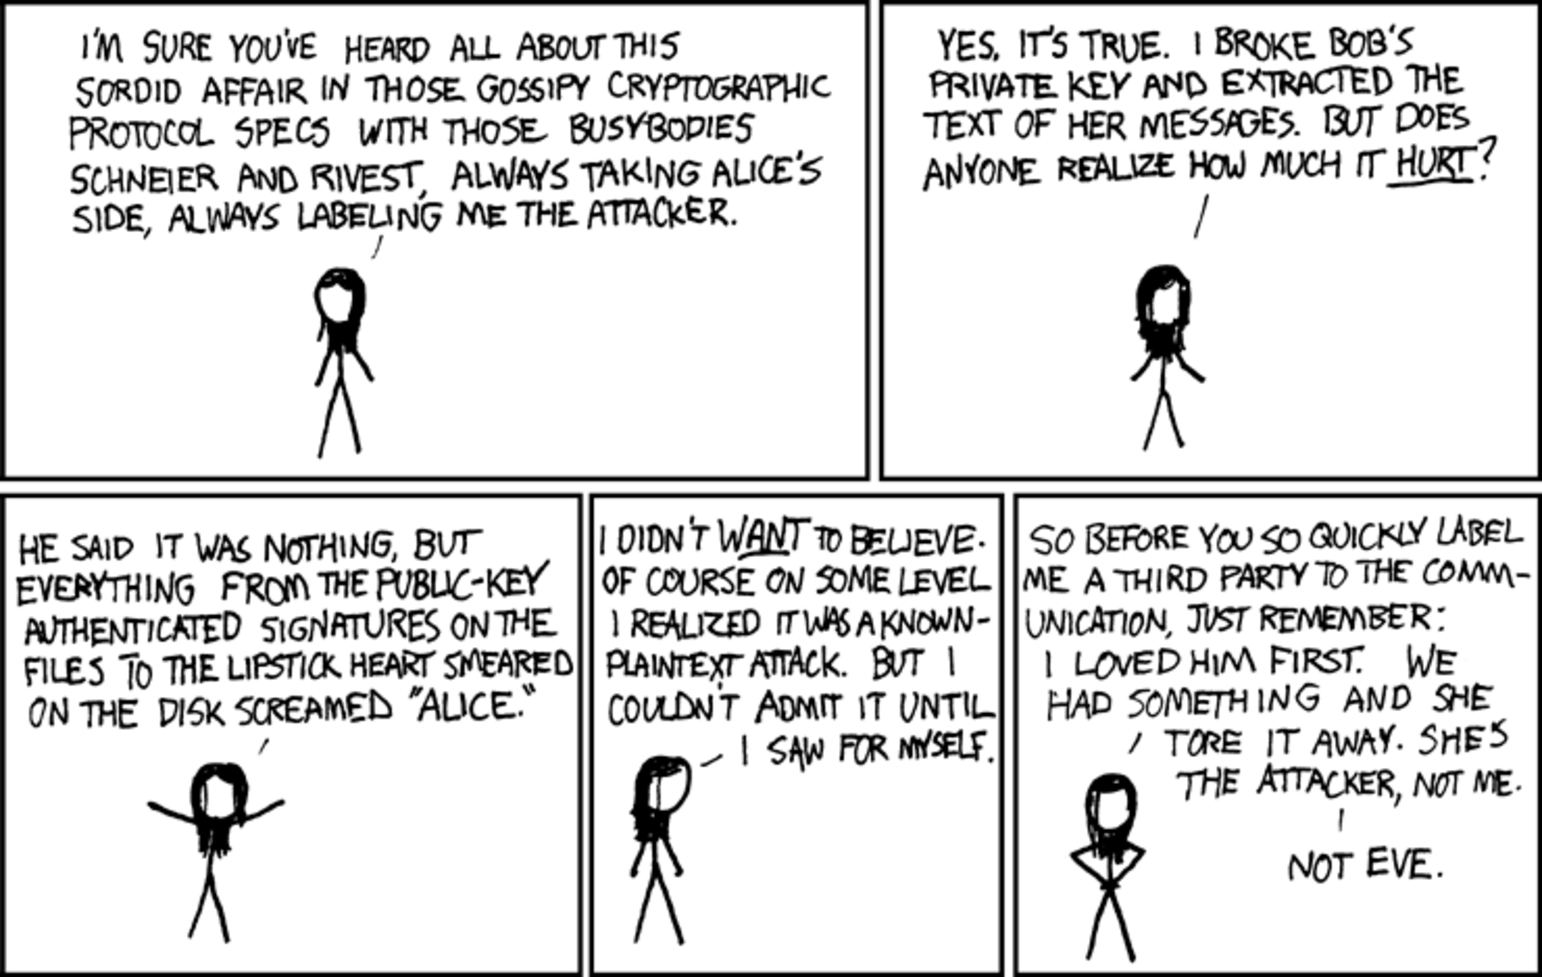
\includegraphics[width=100mm]{pic/term} 
\end{center}
\end{figure}
\end{frame}
\begin{frame}\frametitle{Definitions}
\begin{figure}
\begin{center}
\begin{tikzpicture}
\node (sender) [minimum size=1cm] {}; \Alice{0}{0}{0.4};
\node (bart) [below of = sender, node distance = 0.7cm] {Alice};
\node (enc) [draw, right of = sender, rounded corners=1ex,node distance = 2cm] {$\mathsf{Enc}$};
\node (k1) [above of = enc, node distance = 1cm] {$pk$};
\node (c) [right of = enc, node distance = 2cm] {$c$};
\node (gen) [draw, above of = c, rounded corners=1ex,node distance = 1cm] {$\mathsf{Gen}$};
\node (adv) [below of = c, node distance = 1cm, minimum size=1cm] {}; \Evil{4cm}{-1cm}{0.4};
\node (burns) [below of = adv, node distance = 0.7cm] {Adversary};
\node (dec) [draw, right of = c, rounded corners=1ex,node distance = 2cm] {$\mathsf{Dec}$};
\node (k2) [above of = dec, node distance = 1cm] {$sk$};
\node (receiver) [right of = dec, node distance = 2cm, minimum size=1cm] {}; \Bob{8cm}{0}{0.4};
\node (lisa) [below of = receiver, node distance = 0.7cm] {Bob};
\draw[-latex] (sender) -- (enc) node [midway, above] {$m$};
\draw (enc) -- (c); \draw[-latex] (c) -- (dec);
\draw[-latex] (dec) -- (receiver) node [midway, above] {$m$};
\draw[-latex] (k1) -- (enc);
\draw[-latex] (gen) -- (k1);
\draw[-latex] (gen) -- (k2);								
\draw[-latex] (k2) -- (dec);
\draw[-latex, dotted] (k1) -- (adv);		
\end{tikzpicture}
\end{center}
\end{figure}
\begin{itemize}
\item \textbf{Key-generation} algorithm: $(pk,sk) \gets \mathsf{Gen}$, key length $\ge n$.
\item  \textbf{Plaintext space} $\mathcal{M}$ is associated with $pk$.
\item \textbf{Encryption} algorithm: $c \gets \mathsf{Enc}_{pk}(m)$.
\item \textbf{Decryption} algorithm: $m:= \mathsf{Dec}_{sk}(c)$, or outputs $\perp$.
\item \textbf{Requirement}: $\Pr[\mathsf{Dec}_{sk}(\mathsf{Enc}_{pk}(m)) = m] \ge 1 - \mathsf{negl}(n)$.
\end{itemize}
\end{frame}
\begin{frame}\frametitle{Security against Eavesdroppers $=$ CPA}
The eavesdropping indistinguishability experiment $\mathsf{PubK}^{\mathsf{eav}}_{\mathcal{A},\Pi}(n)$:
\begin{enumerate}
\item $(pk,sk) \gets \mathsf{Gen}(1^n)$.
\item $\mathcal{A}$ \textbf{is given input $\mathbf{pk}$ and so oracle access to $\mathbf{\mathsf{Enc}_{pk}(\cdot)}$}, outputs $m_0, m_1$ of the same length. 
\item $b \gets \{0,1\}$. $c \gets \mathsf{Enc}_{pk}(m_b)$ (challenge) is given to $\mathcal{A}$.
\item $\mathcal{A}$ \textbf{continues to have access to $\mathbf{\mathsf{Enc}_{pk}(\cdot)}$} and outputs $b'$.
\item If $b' = b$, $\mathcal{A}$ succeeded $\mathsf{PrivK}^{\mathsf{eav}}_{\mathcal{A},\Pi}=1$, otherwise 0.
\end{enumerate}
\begin{definition}
$\Pi$ is \textbf{CPA-secure} if $\forall$ \textsc{ppt} $\mathcal{A}$, $\exists$ $\mathsf{negl}$ such that
\[ \Pr\left[\mathsf{PubK}^{\mathsf{cpa}}_{\mathcal{A},\Pi}(n)=1\right] \le \frac{1}{2} + \mathsf{negl}(n). \]
\end{definition}
\end{frame}
\begin{frame}\frametitle{Security Properties of Public-Key Encryption}
%\begin{exampleblock}{} Symmetric ciphers are possible to encrypt a 32-bit message and obtain a 32-bit ciphertext (e.g. with the one time pad). Can the same be done with a public-key system?
%\end{exampleblock}
\begin{theorem}
\alert{Q: Would a deterministic public-key encryption scheme be secure in the presence of an eavesdropper?}
\end{theorem}
\begin{proposition}
\alert{Q: If $\Pi$ is secure in the presence of an eavesdropper, is $\Pi$ also CPA-secure? and is it secure for multiple encryptions?}
\end{proposition}
\begin{proposition}
\alert{Q: Is perfectly-secret public-key encryption possible?}
\end{proposition}
\end{frame}

\begin{comment}
\begin{frame}\frametitle{Definition of Security of Multiple Encryptions}
The multiple message eavesdropping experiment $\mathsf{PubK}^{\mathsf{mult}}_{\mathcal{A},\Pi}(n)$:
\begin{enumerate}
\item $(pk,sk) \gets \mathsf{Gen}(1^n)$.
\item $\mathcal{A}$ is given input $pk$, outputs $\vec{M}_0=(m_0^1,\dots,m_0^t)$, $\vec{M}_1=(m_1^1,\dots,m_1^t)$ with $\forall i, |m_0^i| = |m_1^i|$. 
\item $b \gets \{0,1\}$. $c^i \gets \mathsf{Enc}_{pk}(m_b^i)$ and $\vec{C}=(c^1,\dots,c^t)$ is given to $\mathcal{A}$. $\mathcal{A}$ outputs $b'$.
\item If $b' = b$, $\mathcal{A}$ succeeded $\mathsf{PrivK}^{\mathsf{mult}}_{\mathcal{A},\Pi}=1$, otherwise 0.
\end{enumerate}
\begin{definition}
$\Pi$ has \textbf{indistinguishable multiple encryption in the presence of an eavesdropper} if $\forall$ \textsc{ppt} $\mathcal{A}$, $\exists$ $\mathsf{negl}$ such that
\[ \Pr\left[\mathsf{PubK}^{\mathsf{mult}}_{\mathcal{A},\Pi}(n)=1\right] \le \frac{1}{2} + \mathsf{negl}(n). \]
\end{definition}
\end{frame}
\begin{frame}\frametitle{Security of Two Encryptions}
Prove: for two encryptions, $\Pr[\mathsf{PubK}^{\mathsf{mult}}_{\mathcal{A},\Pi}(n)=1] \le \frac{1}{2} + \mathsf{negl}(n)$.\\ Let $c_i^j = \mathsf{Enc}_{pk}(m_i^j)$.
\begin{align*}
\Pr[\mathsf{PubK}^{\mathsf{mult}}_{\mathcal{A},\Pi}(n)=1] &= \frac{1}{2}\cdot \Pr[\mathcal{A}(\alert{c^1_0},\alert{c^2_0})=\alert{0}] + \frac{1}{2}\cdot \Pr[\mathcal{A}(c^1_1,c^2_1)=1]
\end{align*}
Reduce $\mathcal{A}'$ for a single message to $\mathcal{A}$ for two messages.
\begin{figure}
\begin{center}
\begin{tikzpicture}
\draw (0,0) rectangle (5,4);
\draw (4.25,0.2) rectangle (4.75,3);
\draw[-latex] (-2.5,3.5) -- (0,3.5) node [midway, above] {$pk$};
\draw[-latex] (0,2.5) -- (-2.5,2.5) node [midway, above] {$m_0^2,m_1^2$};
\draw[-latex] (-2.5,1.5) -- (0,1.5) node [midway, above] {$c^2_b$};
\draw[-latex] (0,0.5) -- (-2.5,0.5) node [midway, above] {$b'$};
\draw (1,3.5) node {{\Large $\mathcal{A}'$}};
\draw (4.5,1.75) node {\Large $\mathcal{A}$};
\draw[-latex] (4.25,2.5) -- (0.5,2.5) node [midway, above] {$(m^1_0,m^2_0), (m^1_1,m^2_1)$};
\draw[-latex] (0.5,1.45) -- (4.25,1.45) node [midway, above] {$(c_0^1,c^2_b)$};
\draw[-latex] (4.25,0.5) -- (0.5,0.5) node [midway, above] {$b'$};
\draw[-latex] (4.5,3.5) node[above] {$pk$} -- (4.5,3);
\end{tikzpicture}
\end{center}
\end{figure}
\end{frame}
\begin{frame}\frametitle{Proof (Cont.)}
\[\text{Prove}:\;\frac{1}{2}+\mathsf{negl}(n) \ge \frac{1}{2}\cdot \Pr[\mathcal{A}(\alert{c_0^1},\alert{c_0^2})=\alert{0}] + \frac{1}{2}\cdot \Pr[\mathcal{A}(\alert{c_0^1},c_1^2)=1].\]
$\Pr[\mathcal{A}'(\alert{c^2_0})=\alert{0}]=\Pr[\mathcal{A}(\alert{c^1_0},\alert{c^2_0})=\alert{0}]$;
$\Pr[\mathcal{A}'(c^2_1)=1]=\Pr[\mathcal{A}(\alert{c^1_0},c^2_1)=1]$.\\
\begin{align*}
\frac{1}{2}+\mathsf{negl}(n) &\ge \Pr[\mathsf{PubK}^{\mathsf{eav}}_{\mathcal{A'},\Pi}(n)=1] \\
&= \frac{1}{2}\cdot \Pr[\mathcal{A}'(\alert{c^2_0})=\alert{0}] + \frac{1}{2}\cdot \Pr[\mathcal{A}'(c^2_1)=1]\\
&= \frac{1}{2}\cdot \Pr[\mathcal{A}(\alert{c^1_0},\alert{c^2_0})=\alert{0}] + \frac{1}{2}\cdot \Pr[\mathcal{A}(\alert{c^1_0},c^2_1)=1].
\end{align*}
\[\text{Similarly, }\;\frac{1}{2}+\mathsf{negl}(n) \ge \frac{1}{2}\cdot \Pr[\mathcal{A}(\alert{c_0^1},c_1^2)=\alert{0}] + \frac{1}{2}\cdot \Pr[\mathcal{A}(c_1^1,c_1^2)=1].\]
\end{frame}
\begin{frame}\frametitle{Proof (Cont.)}
\begin{align*}
1+\mathsf{negl}(n) &\ge \frac{1}{2}\cdot \Pr[\mathcal{A}(\alert{c_0^1},\alert{c_0^2})=\alert{0}] + \frac{1}{2}\cdot \Pr[\mathcal{A}(c_1^1,c_1^2)=1]\\
&+ \frac{1}{2}\cdot \left(\Pr[\mathcal{A}(\alert{c_0^1},c_1^2)=1] +  \Pr[\mathcal{A}(\alert{c_0^1},c_1^2)=\alert{0}]\right)\\
&= \frac{1}{2} + \Pr[\mathsf{PubK}^{\mathsf{mult}}_{\mathcal{A},\Pi}(n)=1]. 
\end{align*}
\end{frame}
\begin{frame}\frametitle{Hybrid Argument}
Proof technique to show that two distributions are computationally indistinguishable.
\begin{enumerate}
\item Define a sequence of polynomially many distributions $D_1,\dotsc,D_t$ (hybrid distributions) as follows:
\begin{itemize}
\item $D_1$ and $D_t$ are to be shown computationally indistinguishable.
\item Any adjacent distributions $D_i$ and $D_{i+1}$ differ by only one application of a cryptographic primitive.
\end{itemize}
\item It is (comparatively) easier to prove that adjacent distributions are computationally indistinguishable.
\item Since computational indistinguishability is transitive across a polynomial number of distributions, we conclude that $D_1$ and $D_t$ are computationally indistinguishable.
\end{enumerate}
\end{frame}
\begin{frame}\frametitle{Security of Multiple Encryptions}
Step 1: define a sequence of distribution:
\[ \vec{C}^{(i)} \overset{\text{def}}{=} \underbrace{c^1_0,\dotsc,c^i_0}_{i\; \text{terms}},\underbrace{c^{i+1}_1,\dotsc,c^t_1}_{t-i\; \text{terms}}.\]
\[
\Pr[\mathsf{PubK}^{\mathsf{mult}}_{\mathcal{A},\Pi}(n)=1] = \frac{1}{2}\cdot \Pr[\mathcal{A}(\vec{C}^{(t)})=0] + \frac{1}{2}\cdot \Pr[\mathcal{A}(\vec{C}^{(0)})=1]
\]
\end{frame}
\begin{frame}\frametitle{Proof (Cont.)}
Step 2: prove that adjacent distributions are indistinguishable.\\ Reduce $\mathcal{A}'$ for single message to $\mathcal{A}$.
\begin{figure}
\begin{center}
\begin{tikzpicture}
\draw (0,0) rectangle (5,4);
\draw (4.25,0.2) rectangle (4.75,3);
\draw[-latex] (-2.5,3.5) -- (0,3.5) node [midway, above] {$pk$};
\draw[-latex] (0,2.5) -- (-2.5,2.5) node [midway, above] {$m_0^i,m_1^i$};
\draw[-latex] (-2.5,1.5) -- (0,1.5) node [midway, above] {$c^i_b$};
\draw[-latex] (0,0.5) -- (-2.5,0.5) node [midway, above] {$b'$};
\draw (1,3.5) node {{\Large $\mathcal{A}'$}};
\node at (3,3.5) {$i \gets \{1,\dotsc,t\}$};
\draw (4.5,1.75) node {\Large $\mathcal{A}$};
\draw[-latex] (4.25,2.5) -- (0.5,2.5) node [midway, above] {$\vec{M}_0, \vec{M}_1$};
\draw[-latex] (0.5,1.45) -- (4.25,1.45) node [midway, above] {$\vec{C}^{(i-b)}$};
\draw[-latex] (4.25,0.5) -- (0.5,0.5) node [midway, above] {$b'$};
\draw[-latex] (4.5,3.5) node[above] {$pk$} -- (4.5,3);
\end{tikzpicture}
\end{center}
\end{figure}
If $\mathcal{A}$ distinguishes between $\vec{C}^{(i)}$ and $\vec{C}^{(i-1)}$, this means that it distinguishes between $c^i_0$ and $c^i_1$ (this is the only difference).
\end{frame}
\begin{frame}\frametitle{Proof (Cont.)}
\begin{align*}
\Pr[\mathcal{A'}=0|b=0] &= \sum^t_{i^*=1}\frac{1}{t}\cdot \Pr[\mathcal{A}(\vec{C}^{(i^*)})=0].\\
\Pr[\mathcal{A'}=1|b=1] &= \sum^t_{i^*=1}\frac{1}{t}\cdot \Pr[\mathcal{A}(\vec{C}^{(i^*-1)})=1]\\
&=\sum^{t-1}_{i^*=0}\frac{1}{t}\cdot \Pr[\mathcal{A}(\vec{C}^{(i^*)})=1].
\end{align*}
\end{frame}
\begin{frame}\frametitle{Proof (Cont.)}
Step 3: conclusion.
\begin{align*}
\frac{1}{2}+\mathsf{negl}(n) &\ge \Pr[\mathsf{PubK}^{\mathsf{eav}}_{\mathcal{A'},\Pi}(n)=1] \\
&= \frac{1}{2}\cdot \Pr[\mathcal{A'}=0|b=0] + \frac{1}{2}\cdot \Pr[\mathcal{A'}=1|b=1]\\
&= \sum^t_{i^*=1}\frac{1}{2t}\cdot \Pr[\mathcal{A}(\vec{C}^{(i^*)})=0] + \sum^{t-1}_{i^*=0}\frac{1}{2t}\cdot \Pr[\mathcal{A}(\vec{C}^{(i^*)})=1]\\
&= \frac{1}{2t}\cdot \sum^{t-1}_{i^*=1}\left( \Pr[\mathcal{A}(\vec{C}^{(i^*)})=0] + \Pr[\mathcal{A}(\vec{C}^{(i^*)})=1]\right)\\
&+ \frac{1}{2t}\cdot \left( \Pr[\mathcal{A}(\vec{C}^{(t)})=0] + \Pr[\mathcal{A}(\vec{C}^{(0)})=1]\right)\\
&= \frac{t-1}{2t} + \frac{1}{t}\cdot \Pr[\mathsf{PubK}^{\mathsf{mult}}_{\mathcal{A},\Pi}(n)=1].
\end{align*}
\end{frame}
\begin{frame}\frametitle{Encrypting Arbitrary-Length Messages}
$\Pi = (\mathsf{Gen}, \mathsf{Enc}, \mathsf{Dec})$ is an encryption scheme encrypts only 1-bit message.\\
$\Pi'= (\mathsf{Gen}, \mathsf{Enc}', \mathsf{Dec}')$:
\[\mathsf{Enc}'_{pk}(m)=\mathsf{Enc}_{pk}(m_1),\dotsc,\mathsf{Enc}_{pk}(m_t).\]
\begin{proposition}
If $\Pi$ has indistinguishable encryptions in the presence of an eavesdropper, then so does $\Pi'$.
\end{proposition}
\end{frame}
\end{comment}
\begin{frame}\frametitle{Key Size Comparison}
NIST recommends the \textbf{key lengths} (in bits) with comparable security. NIST deems a 112-bit effective key length acceptable for security until the year 2030, but recommends 128-bit or higher key lengths for applications where security is required beyond then.
\newline
\begin{center}
\begin{tabular}{|c|c|c|} \hline
AES & RSA ($N$)/DH ($p$) & ECC (order $q$) \\ \hline	
56 & 512 & 112 \\
80 & 1024 & 160 \\
112 & 2048 & 224 \\
128 & 3072 & 256 \\
192 & 7680 & 384 \\
256 & 15360 & 512 \\ \hline	
\end{tabular}	
\end{center}
\end{frame}
\begin{frame}\frametitle{Construction of Hybrid Encryption}
To speed up the encryption, use private-key encryption $\Pi'$ (data-encapsulation mechanism, DEM) in tandem with public-key encryption $\Pi$ (key-encapsulation mechanism, KEM).
\begin{columns}
\begin{column}{5cm}
\begin{figure}
\begin{center}
\begin{tikzpicture}
\node (f1) [minimum size=1.25cm,rounded corners=1ex,draw] {$\mathsf{Enc}_{pk}$};
\node (f2) at (2.5cm,0) [minimum size=1.25cm,rounded corners=1ex,draw] {$\mathsf{Enc}'_{k}$};
\draw[-latex] (0,1.5cm) node [above] {$k$} -- (f1);
\draw[-latex] (2.5,1.5cm) node [above] {$m$} -- (f2);
\draw[-latex] (-1cm,0) node [left] {$pk$} -- (f1);
\draw[-latex] (f1) -- +(0,-1.5) node [below] {$c_1$};
\draw[-latex] (f2) -- +(0,-1.5) node [below] {$c_2$};
\draw[-latex] (0,1.25) -| (1.25,0) -- (f2);
\end{tikzpicture}
\end{center}
\end{figure}
\end{column}
\begin{column}{5cm}
\begin{construction}
$\Pi^{\mathsf{hy}} = (\mathsf{Gen}^{\mathsf{hy}}, \mathsf{Enc}^{\mathsf{hy}}, \mathsf{Dec}^{\mathsf{hy}})$:
\begin{itemize}
\item $\mathsf{Gen}^{\mathsf{hy}}$: $(pk,sk) \gets \mathsf{Gen}(1^n)$.
\item $\mathsf{Enc}^{\mathsf{hy}}$: $pk$ and $m$. 
\begin{enumerate}
\item $k \gets \{0,1\}^n$.
\item $c_1 \gets \mathsf{Enc}_{pk}(k)$, $c_2 \gets \mathsf{Enc}'_{k}(m)$.
\end{enumerate}
\item $\mathsf{Dec}^{\mathsf{hy}}$: $sk$ and $\langle c_1,c_2\rangle$.
\begin{enumerate}
\item $k := \mathsf{Dec}_{sk}(c_1)$.
\item $m := \mathsf{Dec}'_k(c_2)$.
\end{enumerate}
\end{itemize}
\end{construction}
\end{column}
\end{columns}
\alert{Q: Is hybrid encryption a public-key enc. or a private-key enc. ?}
\end{frame}
\begin{frame}\frametitle{Security of Hybrid Encryption}
\begin{theorem}
If $\Pi$ is a CPA-secure public-key encryption scheme and $\Pi'$ is a private-key encryption scheme that has indistinguishable encryptions in the presence of an eavesdropper, then $\Pi^{\mathsf{hy}}$ is a CPA-secure public-key encryption scheme.
\end{theorem}
\begin{figure}
\begin{center}
\begin{tikzpicture}[font=\small]
\node (pk0) at (0,0) {$\langle pk,\mathsf{Enc}_{pk}(k),\mathsf{Enc}_{k}'(m_0)\rangle$};
\node (pk1) at (6,0) {$\langle pk,\mathsf{Enc}_{pk}(k),\mathsf{Enc}_{k}'(m_1)\rangle$};
\node (k0) at (0,-2) {$\langle pk,\mathsf{Enc}_{pk}(0^n),\mathsf{Enc}_{k}'(m_0)\rangle$};
\node (k1) at (6,-2) {$\langle pk,\mathsf{Enc}_{pk}(0^n),\mathsf{Enc}_{k}'(m_1)\rangle$};
\draw[latex-latex,dotted] (pk0) -- (pk1) node [midway,above] {\footnotesize (by transitivity)};
\draw[latex-latex] (k0) -- (k1) node [midway,below] {\footnotesize (by security of $\Pi'$)};
\draw[latex-latex] (pk0) -- (k0) node [midway,right] {\footnotesize (by security of $\Pi$)};
\draw[latex-latex] (pk1) -- (k1) node [midway,left] {\footnotesize (by security of $\Pi$)};
\end{tikzpicture}
\end{center}
\end{figure}
\end{frame}
\begin{frame}\frametitle{Applications of Hybrid Encryption\footnote{from BonehShuop v0.5}}
\begin{exampleblock}{How do the following applications work by using hybrid encryption?}
\begin{itemize}
\item \textbf{Sharing encrypted files:} In modern file systems, a user (Alice) can store encrypted files to which other users (Bob, Charlie) have read access. 
\item \textbf{Key escrow:} Consider a company that deploys an encrypted file system such as the one described above. The company runs a key escrow server which generates a public key pair. One day Alice is traveling, but her manager Bob needs to read one of her files to prepare for a meeting. 
\end{itemize}
\end{exampleblock}
\end{frame}
\section{Trapdoor Permutations}
\begin{frame}\frametitle{Overview}
\textbf{Trapdoor function}: is easy to compute, yet difficult to find its inverse without special info., the ``trapdoor''. (One Way Function with the ``trapdoor'')
\newline

A public-key encryption scheme can be constructed from any trapdoor permutation. (``\emph{Theory and Applications of Trapdoor Functions}'', [Yao, 1982])
\begin{figure}
\begin{center}
\begin{tikzpicture}
\node (x) [circle, minimum size=1.5cm, draw] {$x$};
\node (fx) [circle, draw, right of=x, minimum size=1.5cm, node distance=4cm] {$f(x)$};
\node (hc) at ($(x)+(2cm,-1cm)$) [circle, draw] {$\mathsf{hc}(x)$};
\node (tp) [draw, right of=x, node distance=2cm] {$\mathsf{tp}$};
\node (ez) [above of=tp, node distance=0.5cm, blue] {easy};

\draw[-latex,blue] (x) to [bend left=30,-latex,above] node {easy} (fx);
\draw[-latex,red] (fx) to [bend left=30,-latex,right] node {hard} (hc);
\draw[-latex,blue] (x) to [bend right=30,-latex,left] node {easy} (hc);
\draw[-latex,blue] (fx) -- (tp)  -- (x);
\draw[-latex,red] (fx) to [bend right=-120,-latex,below] node {hard} (x);
\end{tikzpicture}
\end{center}
\end{figure}
\end{frame}
\begin{frame}\frametitle{Families of Functions}
\begin{figure}
\begin{center}
\begin{tikzpicture}[uk/.style={inner sep=1pt, minimum width=15pt, circle},kk/.style={inner sep=1pt, minimum width=15pt, circle}]
\node (X) [ellipse,minimum width=3cm,minimum height=4cm,inner color=blue!40,outer color=blue!10] {}; 
\node (D) [ellipse,minimum width=1.5cm,minimum height=2cm,draw] {}; 
\node (x) [above of=X,node distance=2.2cm] {$\mathcal{D}$}; 
\node (d) [above of=X,node distance=1.2cm] {$\mathcal{D}_I$}; 
\node (Y) [right of=X,ellipse,minimum width=3cm,minimum height=4cm,node distance=6cm,inner color=blue!40,outer color=blue!10] {};
\node (R) [right of=X,ellipse,minimum width=1.5cm,minimum height=2cm,node distance=6cm,draw] {}; 
\node (y) [above of=Y,node distance=2.2cm] {$\mathcal{R}$};
\node (r) [above of=Y,node distance=1.2cm] {$\mathcal{R}_I$}; 
\node (gen) [right of=x,node distance=3cm,rounded corners=1ex,draw] {$\mathsf{Gen}$};
\node (I) [below of=gen,node distance=1cm] {$I$};
\draw[-latex] (gen) -- (I);
\node (f) [single arrow,right of=X,node distance=2.8cm, minimum height=2.5cm, minimum width=2.5cm,single arrow head extend=.05cm,fill=blue!40,path fading=west] {};
\node (samp) [left of=I, node distance=1.5cm,draw,rounded corners=1ex,draw] {$\mathsf{Samp}$};
\draw[-latex] (I) -- (samp);
\node (x1) at ($(X)$) [kk] {$x$};
\draw[-latex] (samp) -- (x1);
\node (y1) at ($(Y)$) [uk] {$y$};
\node (fi) at (I |- f) [draw,rounded corners=1ex,draw] {$f_I$};
\draw[-latex] (x1) -- (fi);
\draw[-latex] (fi) -- (y1);
\draw[-latex] (I) -- (fi);
\node (n) [left of=gen,node distance=1.5cm] {$1^n$};
\draw[-latex] (n) -- (gen);
\end{tikzpicture}

\end{center}
\end{figure}
\begin{definition}
$\Pi = (\mathsf{Gen}, \mathsf{Samp}, f)$ is a \textbf{family of functions} if:
\begin{enumerate}
\item \textbf{Parameter-generation} algorithm: $I \gets \mathsf{Gen}(1^n)$.
\item \textbf{sampling} algorithm: $x \gets \mathsf{Samp}(I)$.
\item The deterministic \textbf{evaluation} algorithm: $y := f_I(x)$.
\end{enumerate}
\end{definition}
\end{frame}
\begin{frame}\frametitle{Definition of Families of Trapdoor Permutations}
A tuple of polynomial-time algorithms $\Pi = (\mathsf{Gen}, \mathsf{Samp}, f, \mathsf{Inv})$ is a \textbf{family of trapdoor permutations (TDP)} if:
\begin{itemize}
\item \textbf{parameter generation} algorithm $\mathsf{Gen}$, on input $1^n$, outputs $(I,\mathsf{td})$ with $\abs{I} \ge n$. $(I, \mathsf{td})$ defines a set $\mathcal{D}_I = \mathcal{D}_{\mathsf{td}}$.
\item $\mathsf{Gen}_I$ outputs only $I$.
$(\mathsf{Gen}_I, \mathsf{Samp}, f)$ is OWP.
\item deterministic \textbf{inverting algorithm} $\mathsf{Inv}$. $\forall (I,\mathsf{td})$ and $\forall x \in \mathcal{D}_{I}$, 
\[ \mathsf{Inv}_{\mathsf{td}}(f_I(x))=x.\]
\end{itemize}
Deterministic polynomial-time algorithm $\mathsf{hc}$ is a \textbf{hard-core predicate} of $\Pi$ if $\forall$ \textsc{ppt} $\mathcal{A}$, $\exists$ $\mathsf{negl}$ such that
\[ \Pr[\mathcal{A}(I,f_I(x)) = \mathsf{hc}_I(x)] \le \frac{1}{2} +\mathsf{negl}(n). \]
\end{frame}
\begin{frame}\frametitle{Examples}
\begin{exampleblock}{Let $f$ with $<I, \mathsf{td}>$ be a TDP. Which of the following $f'$ is also a TDP?}
\begin{itemize}
%\item $f'(x) = f(x)\| 000$
\item $f'(x) = f(x)\| \mathsf{td}$
\item $f'(x) = f(x) \| I$
\item $f'(x\|x') = f(x)\|\mathsf{Inv}_{\mathsf{td}}(f(x'))$
\item $f'(x\|x') = f(x)\|f(x')$
\item $ f'(x) = \left\{
  \begin{array}{l l}
    f(x) & \quad \text{if $x[0,1,2,3] \neq 1010$}\\
    x & \quad \text{otherwise}\\
  \end{array} \right. $
\end{itemize}
\end{exampleblock}
\begin{exampleblock}{Is the following public-key encryption scheme from any TDP is secure?}
$\mathsf{Enc}_{I}(m) = f_I(m)$, $\mathsf{Dec}_{\mathsf{td}}(c) = f^{-1}_I(c)$.
\end{exampleblock}
\end{frame}
\begin{frame}\frametitle{Public-key Encryption Schemes from TDPs}
\begin{construction}
\begin{itemize}
\item $\mathsf{Gen}$: $(I, \mathsf{td}) \gets \widehat{Gen}$ output \textbf{public key} $I$ and \textbf{private key} $\mathsf{td}$.
\item $\mathsf{Enc}$: on input $I$ and $m \in \{0,1\}$, choose a random $x\gets \mathcal{D}_I$ and output $\langle f_I(x), \mathsf{hc}_I(x)\oplus m \rangle$.
\item $\mathsf{Dec}$: on input $\mathsf{td}$ and $\langle y, m'\rangle$, compute $x:= f^{-1}_I(y)$ and output $\mathsf{hc}_I(x)\oplus m'$.
\end{itemize}
\end{construction}
\begin{theorem}
If $\widehat{\Pi}=(\widehat{Gen},f)$ is TDP, and $\mathsf{hc}$ is HCP for $\widehat{\Pi}$, then Construction $\Pi$ is CPA-secure.
\end{theorem}
\end{frame}
\begin{frame}\frametitle{Proof}
\textbf{Idea}: $\mathsf{hc}_I(x)$ is pseudorandom. Reduce $\mathcal{A}_{\mathsf{hc}}$ for $\mathsf{hc}$ to $\mathcal{A}$ for $\Pi$.
\begin{figure}
\begin{center}
\begin{tikzpicture}
\draw (0,0) rectangle (5,4);
\draw (4.25,0.2) rectangle (4.75,3);
\draw[-latex] (-2.5,3.5) -- (0,3.5) node [midway, above] {$I$} node [midway, below] {$y \in \mathcal{D}_I$};
%\draw[-latex] (-2.5,2) -- (0,2) node [midway, above] {$g^3 = g^z$ or $g^{xy}$};
%\draw[-latex] (-2.5,1.5) -- (0,1.5) node [midway, above] {$c^2_b$};
\draw[-latex] (4,3.5) node [left] {$pk=I$} -| (4.5,3);
\draw[-latex] (0,0.5) -- (-2.5,0.5) node [midway, above] {$z$ if $b'=b$} node [midway, below] {$\overline{z}$ otherwise};
\draw (1,3.5) node {{\Large $\mathcal{A}_{\mathsf{hc}}$}};
\draw (4.5,1.75) node {\Large $\mathcal{A}$};
\draw[-latex] (4.25,2.5) -- (0.5,2.5) node [midway, above] {$m_0 \neq m_1 \in \{0,1\}$};
\draw (1.5,1.45) node [above] {$b,z \gets \{0,1\}$} node [below] {$ m' := m_b\oplus z$};
\draw[-latex] (3,1.45) -- (4.25,1.45) node [midway, above] {$y, m'$};
\draw[-latex] (4.25,0.5) -- (3,0.5) node [midway, above] {$b'$};
%\draw[-latex] (4.5,3.5) node[above] {$pk$} -- (4.5,3);
\end{tikzpicture}
\end{center}
\end{figure}
\[\Pr[\mathcal{A}_{\mathsf{hc}}(I,f_I(x))=\mathsf{hc}_I(x)] = \]
\[\frac{1}{2}\cdot (\Pr[b'=b|z=\mathsf{hc}_I(x)]+\Pr[b'\neq b|z\neq \mathsf{hc}_I(x)]).\]
\end{frame}
\begin{frame}\frametitle{Proof (Cont.)}
\[\Pr[b'=b|z=\mathsf{hc}_I(x)] = \Pr[\mathsf{PubK}^{\mathsf{eav}}_{\mathcal{A},\Pi}(n)=1]=\varepsilon(n).\]
If $z \neq \mathsf{hc}_I(x)$, $m' = m_b\oplus \overline{\mathsf{hc}}_I(x) = m_{\overline{b}}\oplus \mathsf{hc}_I(x)$,\\ which means $m_{\overline{b}}$ is encrypted.
\[\Pr[b'=b|z\neq \mathsf{hc}_I(x)] = \Pr[\mathsf{PubK}^{\mathsf{eav}}_{\mathcal{A},\Pi}(n)=0]=1-\varepsilon(n).\]
\[\Pr[b'\neq b|z\neq \mathsf{hc}_I(x)] =\varepsilon(n).\]
\[\Pr[\mathcal{A}_{\mathsf{hc}}(I,f_I(x))=\mathsf{hc}_I(x)] = \frac{1}{2}\cdot (\varepsilon(n)+\varepsilon(n)) = \varepsilon(n).\]
\end{frame}
%\begin{frame}\frametitle{Encrypting Longer Messages}
%\begin{theorem}
%If $\exists$ TDP $\Pi$, then $\exists$ TDP $\widehat{\Pi}$ with a HCP $\mathsf{hc}$ for $\widehat{\Pi}$.
%\end{theorem}
%\textbf{Example}: If RSA assumption holds then the least-significant bit is hard-core for the RSA family of TDP.
%\newline
%
%an $\ell$-it message $m=m_1\cdots m_{\ell}$, the public key $I$, the ciphertext is
%\[\langle f_I(x_1), \mathsf{hc}_I(x_I)\oplus m_1\rangle,\dotsc,\langle f_I(x_{\ell}), \mathsf{hc}_I(x_{\ell})\oplus m_{\ell}\rangle,\]
%with $x_1,\dotsc,x_{\ell}$ chosen independently and \emph{u.r.a} from $\mathcal{D}_I$.
%\newline
%
%An alternative way: $x_1\gets \mathcal{D}_I$ and compute $x_{i+1} := f_I(x_i)$ for $i=1$ to $\ell$. the ciphertext is 
%\[\langle x_{\ell+1},\mathsf{hc}_I(x_1)\oplus m_1,\dotsc,\mathsf{hc}_I(x_{\ell})\oplus m_{\ell}\rangle.\]
%\end{frame}
\section{Security Against Chosen-Ciphertext Attacks}
\begin{frame}\frametitle{Scenarios of CCA in Public-Key Setting}
\begin{enumerate}
\item An adversary $\mathcal{A}$ observes the ciphertext $c$ sent by $\mathcal{S}$ to $\mathcal{R}$.
\item $\mathcal{A}$ send $c'$ to $\mathcal{R}$ in the name of $\mathcal{S}$ or its own.
\item $\mathcal{A}$ infer $m$ from the decryption of $c'$ to $m'$.
\end{enumerate}
\begin{exampleblock}{Scenarios}
\begin{itemize}
\item \textbf{login to on-line bank with the password}: trial-and-error, learn info from the feedback of bank.
\item \textbf{reply an e-mail with the quotation of decrypted text}.
\item \textbf{malleability of ciphertexts}: e.g. doubling others' bids at an auction.
\end{itemize}
\end{exampleblock}
\end{frame}
\begin{frame}\frametitle{Definition of Security Against CCA/CCA2}
The CCA/CCA2 indistinguishability experiment $\mathsf{PubK}^{\mathsf{cca}}_{\mathcal{A},\Pi}(n)$:
\begin{enumerate}
\item $(pk,sk) \gets \mathsf{Gen}(1^n)$.
\item $\mathcal{A}$ \textbf{is given input $pk$ and oracle access to $\mathsf{Dec}_{sk}(\cdot)$}, outputs $m_0, m_1$ of the same length. 
\item $b \gets \{0,1\}$. $c \gets \mathsf{Enc}_{pk}(m_b)$ is given to $\mathcal{A}$.
\item $\mathcal{A}$ \textbf{have access to $\mathsf{Dec}_{sk}(\cdot)$ except for $c$ in CCA2}\footnote{CCA is also called Lunchtime attacks; CCA2 is also called Adaptive CCA.} and outputs $b'$.
\item If $b' = b$, $\mathcal{A}$ succeeded $\mathsf{PrivK}^{\mathsf{cca}}_{\mathcal{A},\Pi}=1$, otherwise 0.
\end{enumerate}
\begin{definition}
$\Pi$ has \textbf{CCA/CCA2-secure} if $\forall$ \textsc{ppt} $\mathcal{A}$, $\exists$ $\mathsf{negl}$ such that
\[ \Pr\left[\mathsf{PubK}^{\mathsf{cca}}_{\mathcal{A},\Pi}(n)=1\right] \le \frac{1}{2} + \mathsf{negl}(n). \]
\end{definition}
\end{frame}
\begin{frame}\frametitle{Examples}
\begin{exampleblock}{Let $(Gen, E, D)$ be CCA-secure on message space $\{0, 1\}^{128}$. Which of the following is also CCA-secure?}
\begin{itemize}
\item $E'(pk, m) = (E(pk, m), 0^{128})$\\
$D'(sk, (c_{1}, c_{2})) = \left\{ 
  \begin{array}{l l}
    D(sk, c_{1}) & \quad \text{if}\ c_{2} = 0^{128}\\
    \bot &  \quad \text{otherwise}\\
  \end{array} \right. $
\item $E'(pk, m)= (E(pk, m), E(pk, 0^{128}))$\\
$D'(sk, (c_{1}, c_{2})) = D(sk, c_{1})$
\end{itemize}
\end{exampleblock}
\end{frame}
\begin{frame}{State of the Art on CCA2-secure Encryption}
\begin{itemize}
\item \textbf{Zero-Knowledge Proof}: complex, and impractical. (e.g., Dolev-Dwork-Naor)
\item \textbf{Random Oracle} model: efficient, but not realistic (to consider CRHF as RO). (e.g., RSA-OAEP and Fujisaki-Okamoto)
\item \textbf{DDH(Decisional Diffie-Hellman assumption) and UOWHF(Universal One-Way Hashs Function)}: x2 expansion in size, but security proved w/o RO or ZKP (e.g., Cramer-Shoup system).
\end{itemize}
\textbf{CCA2-secure implies Plaintext-aware}: an adversary cannot produce a valid ciphertext without ``knowing'' the plaintext.
\begin{block}{Open problem}
Constructing a CCA2-secure scheme based on RSA problem as efficient as ``Textbook RSA''.
\end{block}
\end{frame}
\section{Public-Key Encryption from TDP in ROM}
%\section{The Random Oracle Methodology}
\begin{frame}\frametitle{Random Oracle Model (ROM) -- Overview}
\begin{itemize}
\item \textbf{Random oracle (RO)}: a truly random function $H$ answers every possible query with a random response.
\begin{itemize}
\item \textbf{Consistent}: If $H$ ever outputs $y$ for an input $x$ ``on-the-fly'', then it always outputs the same answer given the same input.
\item No one ``knows'' the entire function $H$.
\end{itemize}
\item \textbf{Random oracle model (ROM)}: the existence of a public RO.
%\item \textbf{Standard Model}: the adversary is only limited by time and computational power.
\item \textbf{Methodology}: for constructing proven security in ROM.
\begin{enumerate}
\item a scheme is designed and proven secure in ROM.
\item Instantiate $H$ with a hash function $\hat{H}$, such as SHA-1.
\end{enumerate}
\item \alert{No one seriously claims that a random oracle exists}.\footnote{There exists schemes that are proven secure in ROM but are insecure no matter how the random oracle is instantiated.}
\end{itemize}
\emph{With ROM, it is easy to achieve proven security, while keeping the efficiency by appropriate instantiation.}
\end{frame}
%\begin{frame}\frametitle{ROM in Detail}
%\begin{itemize}
%\item \textbf{Consistent}: If $H$ ever outputs $y$ for an input $x$ ``on-the-fly'', then it always outputs the same answer given the same input.
%\item No one ``knows'' the entire function $H$.
%\item \textbf{PRF vs. RO}: PRF emulates RO, and has different usage:
%\begin{itemize}
%\item PRF: a way of defining what it means for a concrete keyed function to be pseudorandom.
%\item RO: as part of the construction of the primitive, and so must be instantiated if we want a concrete realization.
%\end{itemize}
%\end{itemize}
%\end{frame}
\begin{frame}\frametitle{Simple Illustrations of ROM}
An RO maps $n_1$-bit inputs to $n_2$-bit outputs.
\begin{itemize}
\item An RO as an OWF, experiment:
\begin{enumerate}
\item A random function $H$ is chosen
\item A random $x \in \{0,1\}^{n_1}$ is chosen, and $y := H(x)$ is evaluated
\item $\mathcal{A}$ is given $y$, and succeeds if it outputs $x'$: $H(x')=y$
\end{enumerate}
\item An RO as a CRHF, experiment:
\begin{enumerate}
\item A random function $H$ is chosen
\item $\mathcal{A}$ succeeds if it outputs $x, x'$ with $H(x)=H(x')$ but $x\neq x'$
\end{enumerate}
\item Constructing a PRF from an RO: $n_1=2n$, $n_2=n$.
$ F_k(x) \overset{\text{def}}{=} H(k\| x),\;\; \abs{k}=\abs{x}=n.$
\end{itemize}
\end{frame}
%\begin{frame}\frametitle{Is the Random Oracle Methodology Sound?}
%\begin{itemize}
%\item \textbf{Pro}:
%\begin{itemize}
%\item enables the design of more efficient schemes.
%\item better than no proof at all.
%\item only possible weaknesses are due to the hash function.
%\item few real-world attacks on ``natural'' secure schemes in ROM.
%\end{itemize}
%\item \textbf{Con}:
%\begin{itemize}
%\item No proof that security in ROM implies real-world security.
%\item The reduction can not see ``queries'' in the real world.
%\item Not well understand what is a ``good'' CRHF/PRF like a RO.
%\end{itemize}
%\end{itemize}
%\begin{itemize}
%\item What does security in the ROM guarantee in the real world?
%\item Are ROM fundamentally different from the standard model?
%\end{itemize}
%\end{frame}
\begin{frame}\frametitle{Security Against CPA}
\textbf{Idea}: PubK CPA = PrivK + (Secret Key = TDP + RO)
\begin{columns}[t]
\begin{column}{5cm}
\begin{figure}[t]
\begin{center}
\begin{tikzpicture}
\node (f1) [rounded corners=1ex,minimum size=0.7cm, draw] {$f_{I}$};
\node (h1) [right of=f1, node distance=1cm, minimum size=0.7cm, rounded corners=1ex, draw] {$H$};
\node (p1) [right of=h1, node distance=1cm, circle, radius=0.5cm, draw] {};
\draw[-] (p1.north) -- (p1.south);
\draw[-] (p1.east) -- (p1.west);

\draw[-latex] (0,1cm) node [above] {$r$} -- (f1);
\draw[-latex] (0,1cm) -| (h1.north);
\draw[-latex] (2,1cm) node [above] {$m$} -- (p1);
\draw[-latex] (-1cm,0) node [left] {$pk$} -- (f1);
\draw[-latex] (h1) -- (p1.west);
\draw[-latex] (f1) -- +(0,-1) node [below] {$c_1$};
\draw[-latex] (p1) -- +(0,-1) node [below] {$c_2$};
\end{tikzpicture}
\end{center}
\end{figure}\end{column}
\begin{column}{5cm}
\begin{construction}
\begin{itemize}
\item $\mathsf{Gen}$: $pk =  I $, $sk = \mathsf{td} $
\item $\mathsf{Enc}$: $r \gets \{0,1\}^*$, output $\langle c_{1}=f_I(r), c_{2}=H(r)\oplus m\rangle$
\item $\mathsf{Dec}$: $r := f_{\mathsf{td}}^{-1}(c_1)$, output $H(r)\oplus c_2$
\end{itemize}
\end{construction}
\end{column}
\end{columns}
\begin{theorem}
If $f$ is TPD and $H$ is RO, Construction is CPA-secure.
\end{theorem}
\alert{$H$ can not be replaced by PRG, since the partial info on $r$ may be leaked by $c_1$.}
\end{frame}

\begin{frame}\frametitle{CCA-secure based on Private Key Encryption}
\textbf{Idea}: PubK CCA = PrivK CCA + (Secret Key = TPD + RO).  

\begin{columns}[t]
\begin{column}{5cm}
\begin{figure}[t]
\begin{center}
\begin{tikzpicture}
\node (f1) [rounded corners=1ex,minimum size=0.7cm, draw] {$f_{I}$};
\node (h1) [right of=f1, node distance=1cm, minimum size=0.7cm, rounded corners=1ex, draw] {$H$};
%\node (p1) [right of=h1, node distance=1cm, circle, radius=0.5cm, draw] {};
%\draw[-] (p1.north) -- (p1.south);
%\draw[-] (p1.east) -- (p1.west);
\node (p1) [right of=h1, node distance=1cm, minimum size=0.7cm, rounded corners=1ex, draw] {$E$};


\draw[-latex] (0,1cm) node [above] {$r$} -- (f1);
\draw[-latex] (0,1cm) -| (h1.north);
\draw[-latex] (2,1cm) node [above] {$m$} -- (p1);
\draw[-latex] (-1cm,0) node [left] {$pk$} -- (f1);
\draw[-latex] (h1) -- (p1.west);
\draw[-latex] (f1) -- +(0,-1) node [below] {$c_1$};
\draw[-latex] (p1) -- +(0,-1) node [below] {$c_2$};
\end{tikzpicture}
\end{center}
\end{figure}\end{column}
\begin{column}{5cm}
\begin{construction}
\begin{itemize}
\item $\Pi'$ is PrivK
\item $\mathsf{Gen}$: $pk = I$, $sk = \mathsf{td}$.
\item $\mathsf{Enc}$: $k := H(r), r \gets D_I$, output $\langle c_1= f_I(r), c_2 = \mathsf{Enc}'_k(m)\rangle$.
\item $\mathsf{Dec}$: $r := f^{-1}_{\mathsf{td}}(c_1)$, $k:=H(r)$, output $\mathsf{Dec}'_k(c_2)$.
\end{itemize}
\end{construction}

\end{column}
\end{columns}


\begin{theorem}
If $f$ is TDP, $\Pi'$ is CCA-secure, and $H$ is RO, Construction is CCA-secure.
\end{theorem}
\end{frame}
\begin{frame}\frametitle{CCA-secure based on TPD in ROM}
\textbf{Idea}: PubK CCA = TDP + 2 RO (one for enc, one for mac)
\begin{columns}[t]
\begin{column}{5cm}
\begin{figure}[t]
\begin{center}
\begin{tikzpicture}
\node (f1) [rounded corners=1ex,minimum size=0.7cm, draw] {$f_{I}$};
\node (h1) [right of=f1, node distance=1cm, minimum size=0.7cm, rounded corners=1ex, draw] {$H$};
\node (p1) [right of=h1, node distance=1cm, circle, radius=0.5cm, draw] {};
\draw[-] (p1.north) -- (p1.south);
\draw[-] (p1.east) -- (p1.west);
\node (g1) [right of=p1, node distance=1cm, minimum size=0.7cm, rounded corners=1ex, draw] {$G$};


\draw[-latex] (0,1cm) node [above] {$r$} -- (f1);
\draw[-latex] (0,1cm) -| (h1.north);
\draw[-latex] (2,1cm) node [above] {$m$} -- (p1);
\draw[-latex] (2,1cm) -| (g1);
\draw[-latex] (-1cm,0) node [left] {$pk$} -- (f1);
\draw[-latex] (h1) -- (p1.west);
\draw[-latex] (f1) -- +(0,-1) node [below] {$c_1$};
\draw[-latex] (p1) -- +(0,-1) node [below] {$c_2$};
\draw[-latex] (p1) -- (g1);
\draw[-latex] (g1) -- +(0,-1) node [below] {$c_3$};
\end{tikzpicture}
\end{center}
\end{figure}\end{column}
\begin{column}{5cm}
\begin{construction}
\begin{itemize}
\item $\mathsf{Gen}$: $pk = I$, $sk = \mathsf{td}$
\item $\mathsf{Enc}$: $r \gets D_I$, output $\langle c_1=f_I(r), c_2 = H(r)\oplus m, c_3=G(c_2\|m)\rangle$
\item $\mathsf{Dec}$: $r := f^{-1}_{\mathsf{td}}(c_1)$, $m := H(r)\oplus c_2$. If $G(c_2\|m) = c_3$ output $m$, otherwise $\perp$
\end{itemize}
\end{construction}
\end{column}
\end{columns}
\begin{theorem}
If $f$ is TDP, $G,H$ are ROs, Construction is CCA-secure.
\end{theorem}
\end{frame}

\begin{frame}\frametitle{Private Key Encryption vs. Public Key Encryption}
\begin{center}
\begin{tabular}{|c|c|c|} \hline
   & \textbf{Private Key} & \textbf{Public Key}             \\ \hline
\textbf{Secret Key}               & both parties & receiver \\ \hline
\textbf{Weakest Attack}           & Eav          & CPA      \\ \hline
\textbf{Probabilistic}            & CPA/CCA      & always   \\ \hline
\textbf{Assumption against CPA}   & OWF          & TDP      \\ \hline
\textbf{Assumption against CCA}   & OWF          & TDP$+$RO   \\ \hline
\textbf{Efficiency}               & fast         & slow     \\ \hline
\end{tabular}	
\end{center}
\end{frame}
\end{document}
